%SIP template made by Melany Diaz, January 2016

\documentclass[12pt]{article}

\author{Melany Diaz}
\title{SIP}
\date{\today}

% math
\usepackage{amsmath,amssymb}
%\usepackage{amsthm} % uncomment to enable theorem environment
\usepackage{listings}%used to present classes and java code
\usepackage{indentfirst}
\usepackage{graphicx}
\graphicspath{{LatexImages/}}
% 1 inch margins
\usepackage[right=1in, top=1in, bottom = 1in, left=1.5in]{geometry}

\usepackage{fancyhdr}
\pagestyle{fancy}
%\lhead{CS 215}
%\chead{Insertion Sort Analysis}
%\rhead{Melany Diaz}

\usepackage[utf8]{inputenc}
\usepackage[english]{babel}

\usepackage{pdfpages}

\usepackage{ragged2e}

\usepackage{float}

\usepackage{tocloft}
\newcommand{\listappendicesname}{\Large{List of Appendices}}
\newlistof{appendices}{apc}{\listappendicesname}
\newcommand{\appendices}[1]{\addcontentsline{apc}{appendices}{#1}}

\parindent0mm

\usepackage{setspace}
\doublespacing

\usepackage{soul} %for strikeout

\begin{document}

	\fancyhf{} % clear all header and footer fields
	\pagenumbering{roman}
	\fancyfoot[C]{\thepage}
	\setcounter{page}{2}
	\section{Preface}
	
	"I had no idea that this was happening around me" He said, as we walked out of a Minorities in Computer Science lecture. "Is there any possible way that I could help? Anything I could do?" He looked at me expectedly.\\
	
	Was he expecting me to know the answer because I was a Latina woman in Computer Science? I couldn't answer him. Mostly because I didn't know that was happening around me (and to me) either. But the farther away we walked from that conference, the more I started to recognize how the topics mentioned at the lecture showed themselves in my life. All of the anecdotes of professional women and people of color driven away from their careers slowly but constantly began to resonate familiarly with some of the experiences I had already had- only shortly after declaring my major in Computer Science.  I couldn't say that the feelings of isolation and inadequacy were on the verge of making me quit my studies, the way that they had forced the professionals in the lecture to leave their careers. The impostor syndromes mentioned at the lecture hadn't yet fostered such impactful forces into my small experience in computer science. But they were beginning to show up enough for me to consider exploring a different major. \\
	
	I remind myself often of how lucky I was to attend that lecture so early on in my computing career. To learn that there were some external factors that had forced people that looked like me to quit their careers in computing science, simply because of how they identified. Early on, I decided to stubbornly stay, to give a different face to the discipline, and grew a passion for computing along the way. \\
	
	I was in no way expected to educate my peer on what he could do to help and aide minorities in computing. We had a pleasant conversation on the topic and moved on. But his question remained in my unconsciousness, what \textit{could} be done? Thus, my SIP.  \\
	
	
	When the idea for this SIP was born, I had dreamed of writing about diversifying the computing field \textit{in general}. Not just specifying the topic to gender. Because of the sheer size of that topic, I quickly realized I had to narrow my topic down, thus this new topic developed. It is very important for me to note, however, that though this paper focuses on eradicating the gender gap in Computer Science and the diversification of the field in terms of gender, this review is written with the understanding that oppressive constructs (racism, sexism, homophobia, transphobia, ableism, xenophobia, classism, etc.) are interconnected and cannot be examined separately from one another. I would also like to mention that due to a lack of preceding research and available data, a lot of the statistics and demographics illustrated in this report tend to conform to the gender binary, or the classification of sex and gender into two distinct, opposite and disconnected forms of masculine and feminine. Though the finalized paper does not reflect this as much as I had hoped, this report was written with the understanding that in order to fully diversify the field, one cannot simply focus on attracting and retaining more women, but rather rewrite the image of the Computer Science industry to reflect a greater diversity.
	
	\pagebreak
	\subsection{Acknowledgements} 		NOTE TO MEL: CHANGE THIS BEFORE FRIDAY
		
	Thank you all so very much. Thank you to the Academy (Street). Thank you to all of you in this room. I have to congratulate the other incredible nominees this year. The \st{Revenant} SIP was the product of the tireless efforts of an unbelievable cast and crew. First off, to my \st{brother}sisters in this endeavor, \st{Mr. Tom Hardy} Mrs. Megan Diaz and Ms. Monica Diaz. \st{Tom}Sisters, your talent on screen can only be surpassed by your friendship off screen … thank you for creating a transcendent cinematic experience. Thank you to everybody at \st{Fox and New Regency} K College … my entire team. I have to thank everyone from the very onset of my career … To my parents; none of this would be possible without you. And to my friends, I love you dearly; you know who you are.\\
	
	And lastly, I just want to say this: Making The \st{Revenant} SIP was about (wo)man's relationship to the \st{natural} Computer world. A world that we collectively felt in 2015 as the hottest year in recorded history. Our production needed to move to the southern tip of this planet just to be able to find snow. Climate change is real, it is happening right now. It is the most urgent threat facing our entire species, and we need to work collectively together and stop procrastinating. We need to support leaders around the world who do not speak for the big polluters, but who speak for all of humanity, for the indigenous people of the world, for the billions and billions of underprivileged people out there who would be most affected by this. For our children’s children, and for those people out there whose voices have been drowned out by the politics of greed. I thank you all for this amazing award tonight. Let us not take this planet for granted. I do not take tonight for granted. Thank you so very much.
	
   \st{Leonardo Dicaprio at the Oscars} 
	
	\pagebreak
	\subsection{Abstract}
	
	Historically, women have played a crucial role in the evolution of computing, dating as far back as the development of programming in the 1800s. Yet even with this strong historical influence, and the fact that women benefit as equally as men from the services of technology, they are not a strong presence in the developing, designing, and creating teams behind the products. This report will explore some of the influences that discourage women to engage in computing careers and education, offer three proven solutions to these disparities, and describe the implementation and results of these three solutions across different platforms. 
	\pagebreak
	
	\tableofcontents
	
	\pagebreak
	
%%	\listoftables
	
	\pagebreak
	
	\listoffigures
	
	\pagebreak
	
	\listofappendices
	
	\pagebreak
	

	\fancyhf{} % clear all header and footer fields
	\pagenumbering{arabic}
	\fancyhead[C]{\thepage}
	
    \section{Research}
	
	\begin{quotation}
		\begin{center}
			\singlespacing
			\textit{“Twenty years ago, a girl could be a secretary, school teacher, a social worker, or a nurse. If she was really ambitious, she could go into the profession and compete with men… usually working harder and longer to earn less pay for the same job. Now come the big, dazzling computers- and a whole new kind of work for women: programming. Telling the miracle machines what to do and how to do it. Anything from predicting the weather to sending out billing notices from the local department store. \\
				And if it doesn’t sound like a woman’s work- well, it just is.” \\
				-Cosmopolitan Magazine, 1967 }\cite{cosmo}
		\end{center}	
	\end{quotation}

	48 years ago, Cosmopolitan Magazine printed an article advertising for a new and lucrative field for women- computer science. The article boasted the high pay grade of the new field, claiming that “a girl senior systems analyst could earn \$20,000 a year – and up!” Considering that in 1967, the average household earned between \$10,000-\$14,999 yearly\cite{income1969},who wouldn’t be tempted to explore such a high-paying new field? Programming and Computer Science were new to the game, and with predecessors like famed Grace Hopper and the early human computers and calculators (another primarily female job) it was natural for these new jobs to be targeting a more feminine audience.\footnote{The Cosmopolitan Magazine article can be found in Appendix A.} \\
	
	Back to the twenty first century, the Glassdoor List of 25 Best Jobs in America for 2016 shows an impressive majority of employment leaning towards the technologies and science\cite{glassdoor}.The list is composed by combining three key factors- number of job openings, salaries, and career opportunities. What started off as a profitable career where an individual could grow and find further opportunities to improve and move up has consistently grown towards an even more profitable (now offering wages of up to \$120,000 or more) and encouraging employment. As the Glassdoor list implies, it has also continued to be a field with a high number of job openings and frequent job listings. In fact, there are so many job openings that the technology field is in the midst of a severe work-force shortage. It is estimated that an estimated 900,000 jobs go unfilled, with over 40 percent of software projects cancelled due to a shortage of skilled workers, causing an estimated \$4 billion loss in Silicon Valley alone\cite{margolis}.\\
	
	With the parameters so encouraging such as strong demand, endless opportunities and high pay, and a history with such a strong female presence, why is it that even 48 years after the initial call for women programmers, the computer sciences are still primarily male? It is estimated that women make up only 18 percent of directors of Silicon Valley’s tech companies. Even more startling, they only make up just 27 percent of the digital workforce\cite{silicon}.\\
	
	Every day, talented women who could make up for the shortage of qualified workers are disaffected or discouraged from pursuing computing careers and the underlying causes of this disaffection are innumerable.	The first section of this paper will research the statistical representation of women in computer science, both as users and developers, followed by an exploration and discovery of a few reasons that may be causing these disparities and some proposed solutions. The second section will describe how the topics found in the research process were used in different platforms and venues to encourage more women to stay in the technologies.\\
	
	
	\pagebreak
	
	\subsection{Statistics and Demographics} %%QUANTIFIERS?
	Despite the relative youth of the computer industry, much of which began with female-oriented human computer careers, evidence shows that women have lost ground in the world of computing. In today's day and age, women are utilizing technology in equal proportions to men. Whether it is using the Internet, taking advantage of wearable technology, or installing a mobile app, women use technology as much as men.  
	
	According to the Pew Research Center, the demographic of Internet users in 2014 was almost equally split between men and women, as the following figures illustrate. \\
	
	\begin{figure}[H]
		\begin{center}
			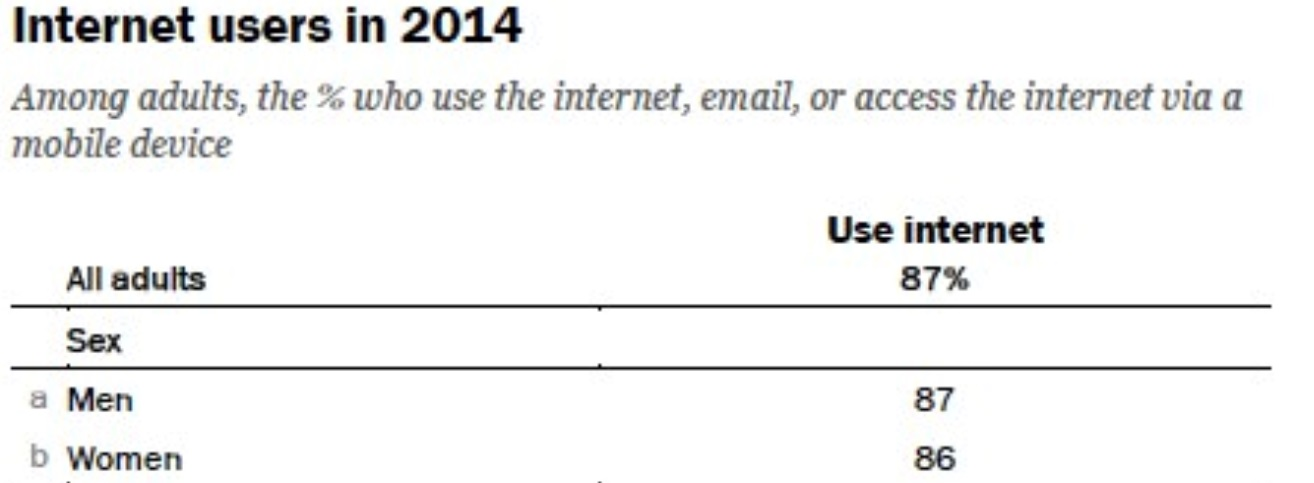
\includegraphics[]{StatsInternet.JPG}
			\caption{Internet Users Categorized by Gender}		
		\end{center}
	\end{figure}
	
		\begin{figure}[H]
			\begin{center}
				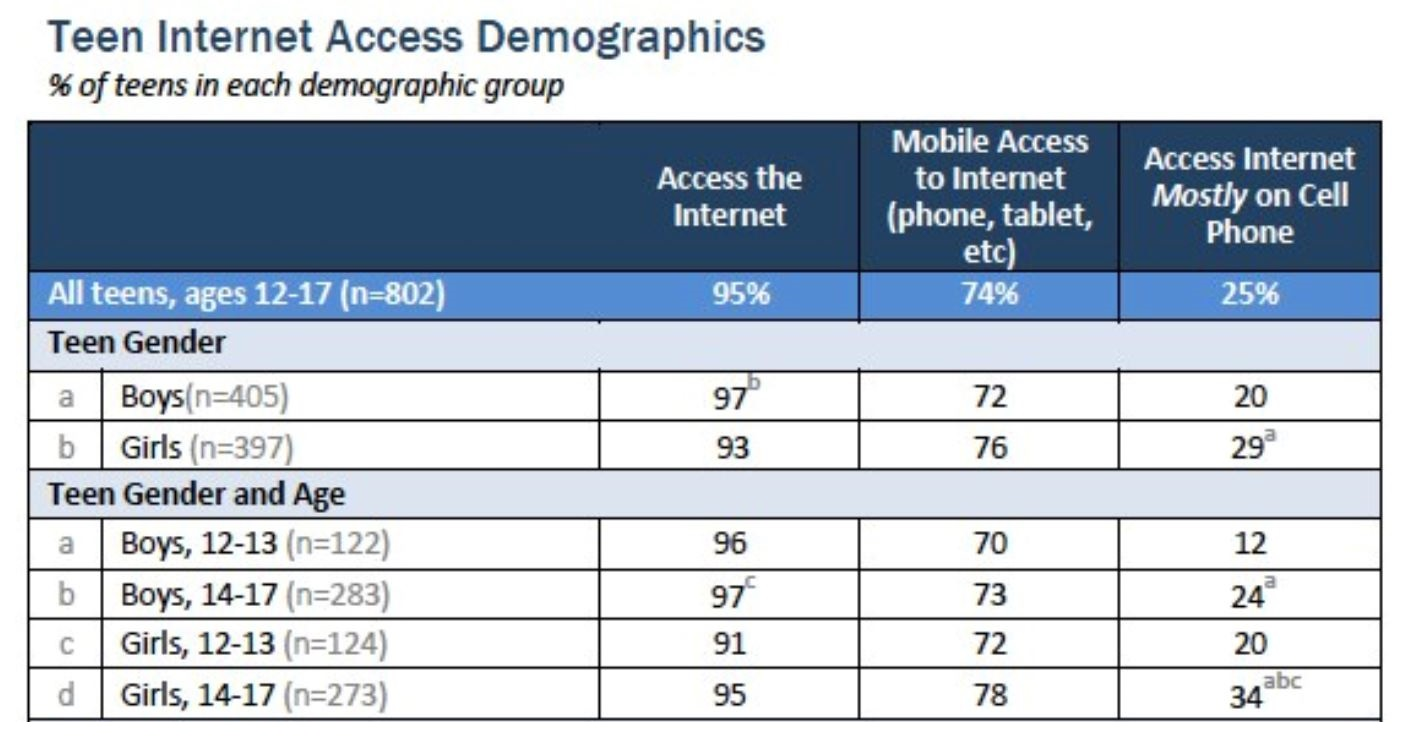
\includegraphics[]{StatsInternet2.JPG}
				\caption{Teen Internet Access Categorized by Gender}		
			\end{center}
		\end{figure}
	
	Furthermore, as can be shown in the following figure, except for the cases of LinkedIn and Twitter, women are a strong majority of social media users.\\
	
	\begin{figure}[H]
		\begin{center}
			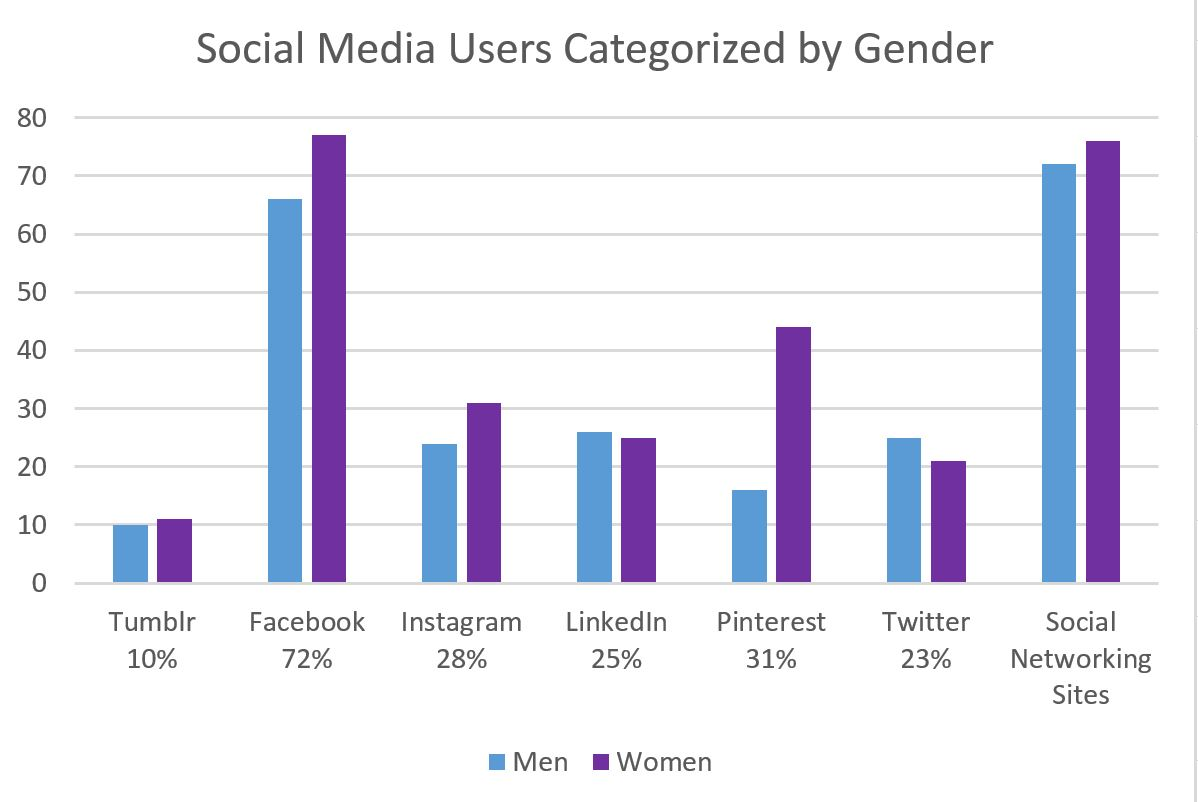
\includegraphics[]{SocialMediaStats}
			\caption{Social Media Users Categorized by Gender}
		\end{center}
	\end{figure}
	
	Though Internet and social media aren't the only sectors were women are equally using technology. Take for example one of the more basic of functions: Messaging. According the the PewResearch Report, even messaging and messaging mobile apps are equally distributed by the genders\\
	
		\begin{figure}[H]
			\begin{center}
				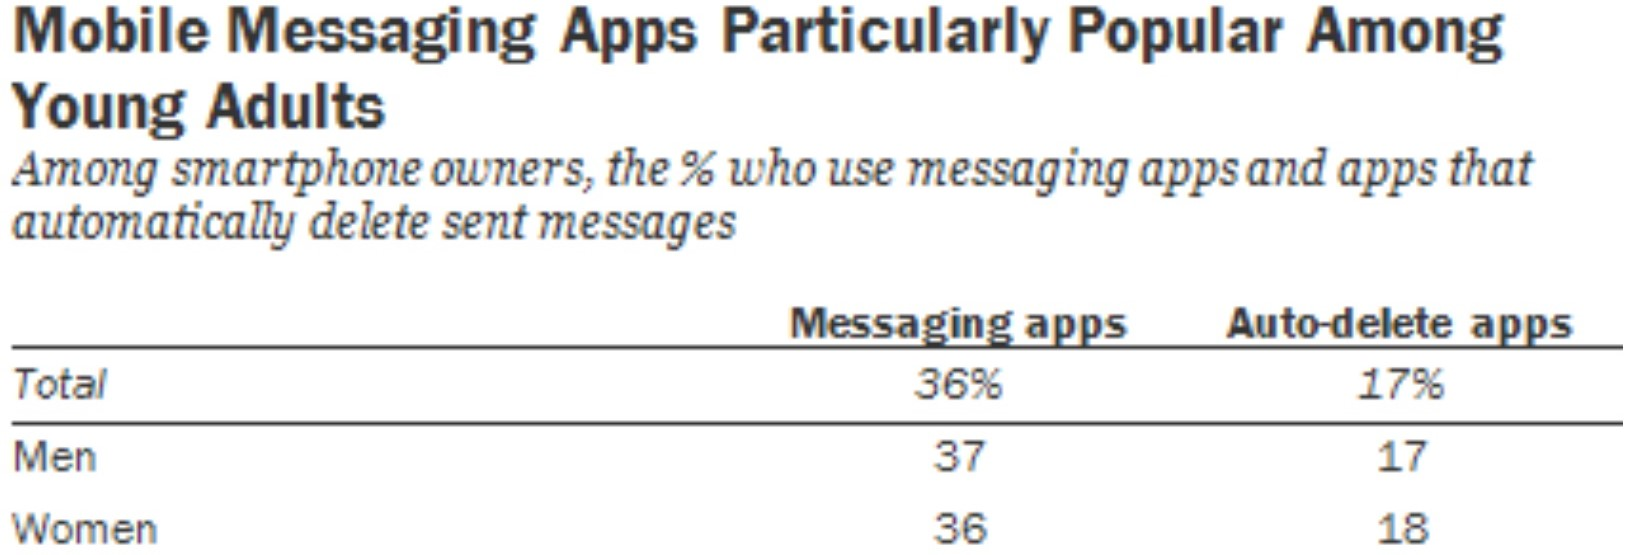
\includegraphics[width=\textwidth,keepaspectratio]{StatsMessaging}
				\caption{Mobile Messaging App Use Categorized by Gender}		
			\end{center}
		\end{figure}
		
	Even in the field of gaming, which is typically thought of as a very masculine and male-oriented market has its fair share of female users. In a report by Developers Magic, developers are encouraged to understand the audience of their games in order to tailor the product better for their consumers. The report divides games and their respective audiences into different categories: Casual and Hard-core. Casual gamers tend to entertain themselves with games when the time presents itself, while Hard-core gamers will arrange their schedules around gaming\cite{gamestats}. Notice the gender differences between a Casual game (Bejeweled Bitz) and a Hard-core game (Call of Duty)
	\\
			\begin{figure}[H]
				\begin{center}
					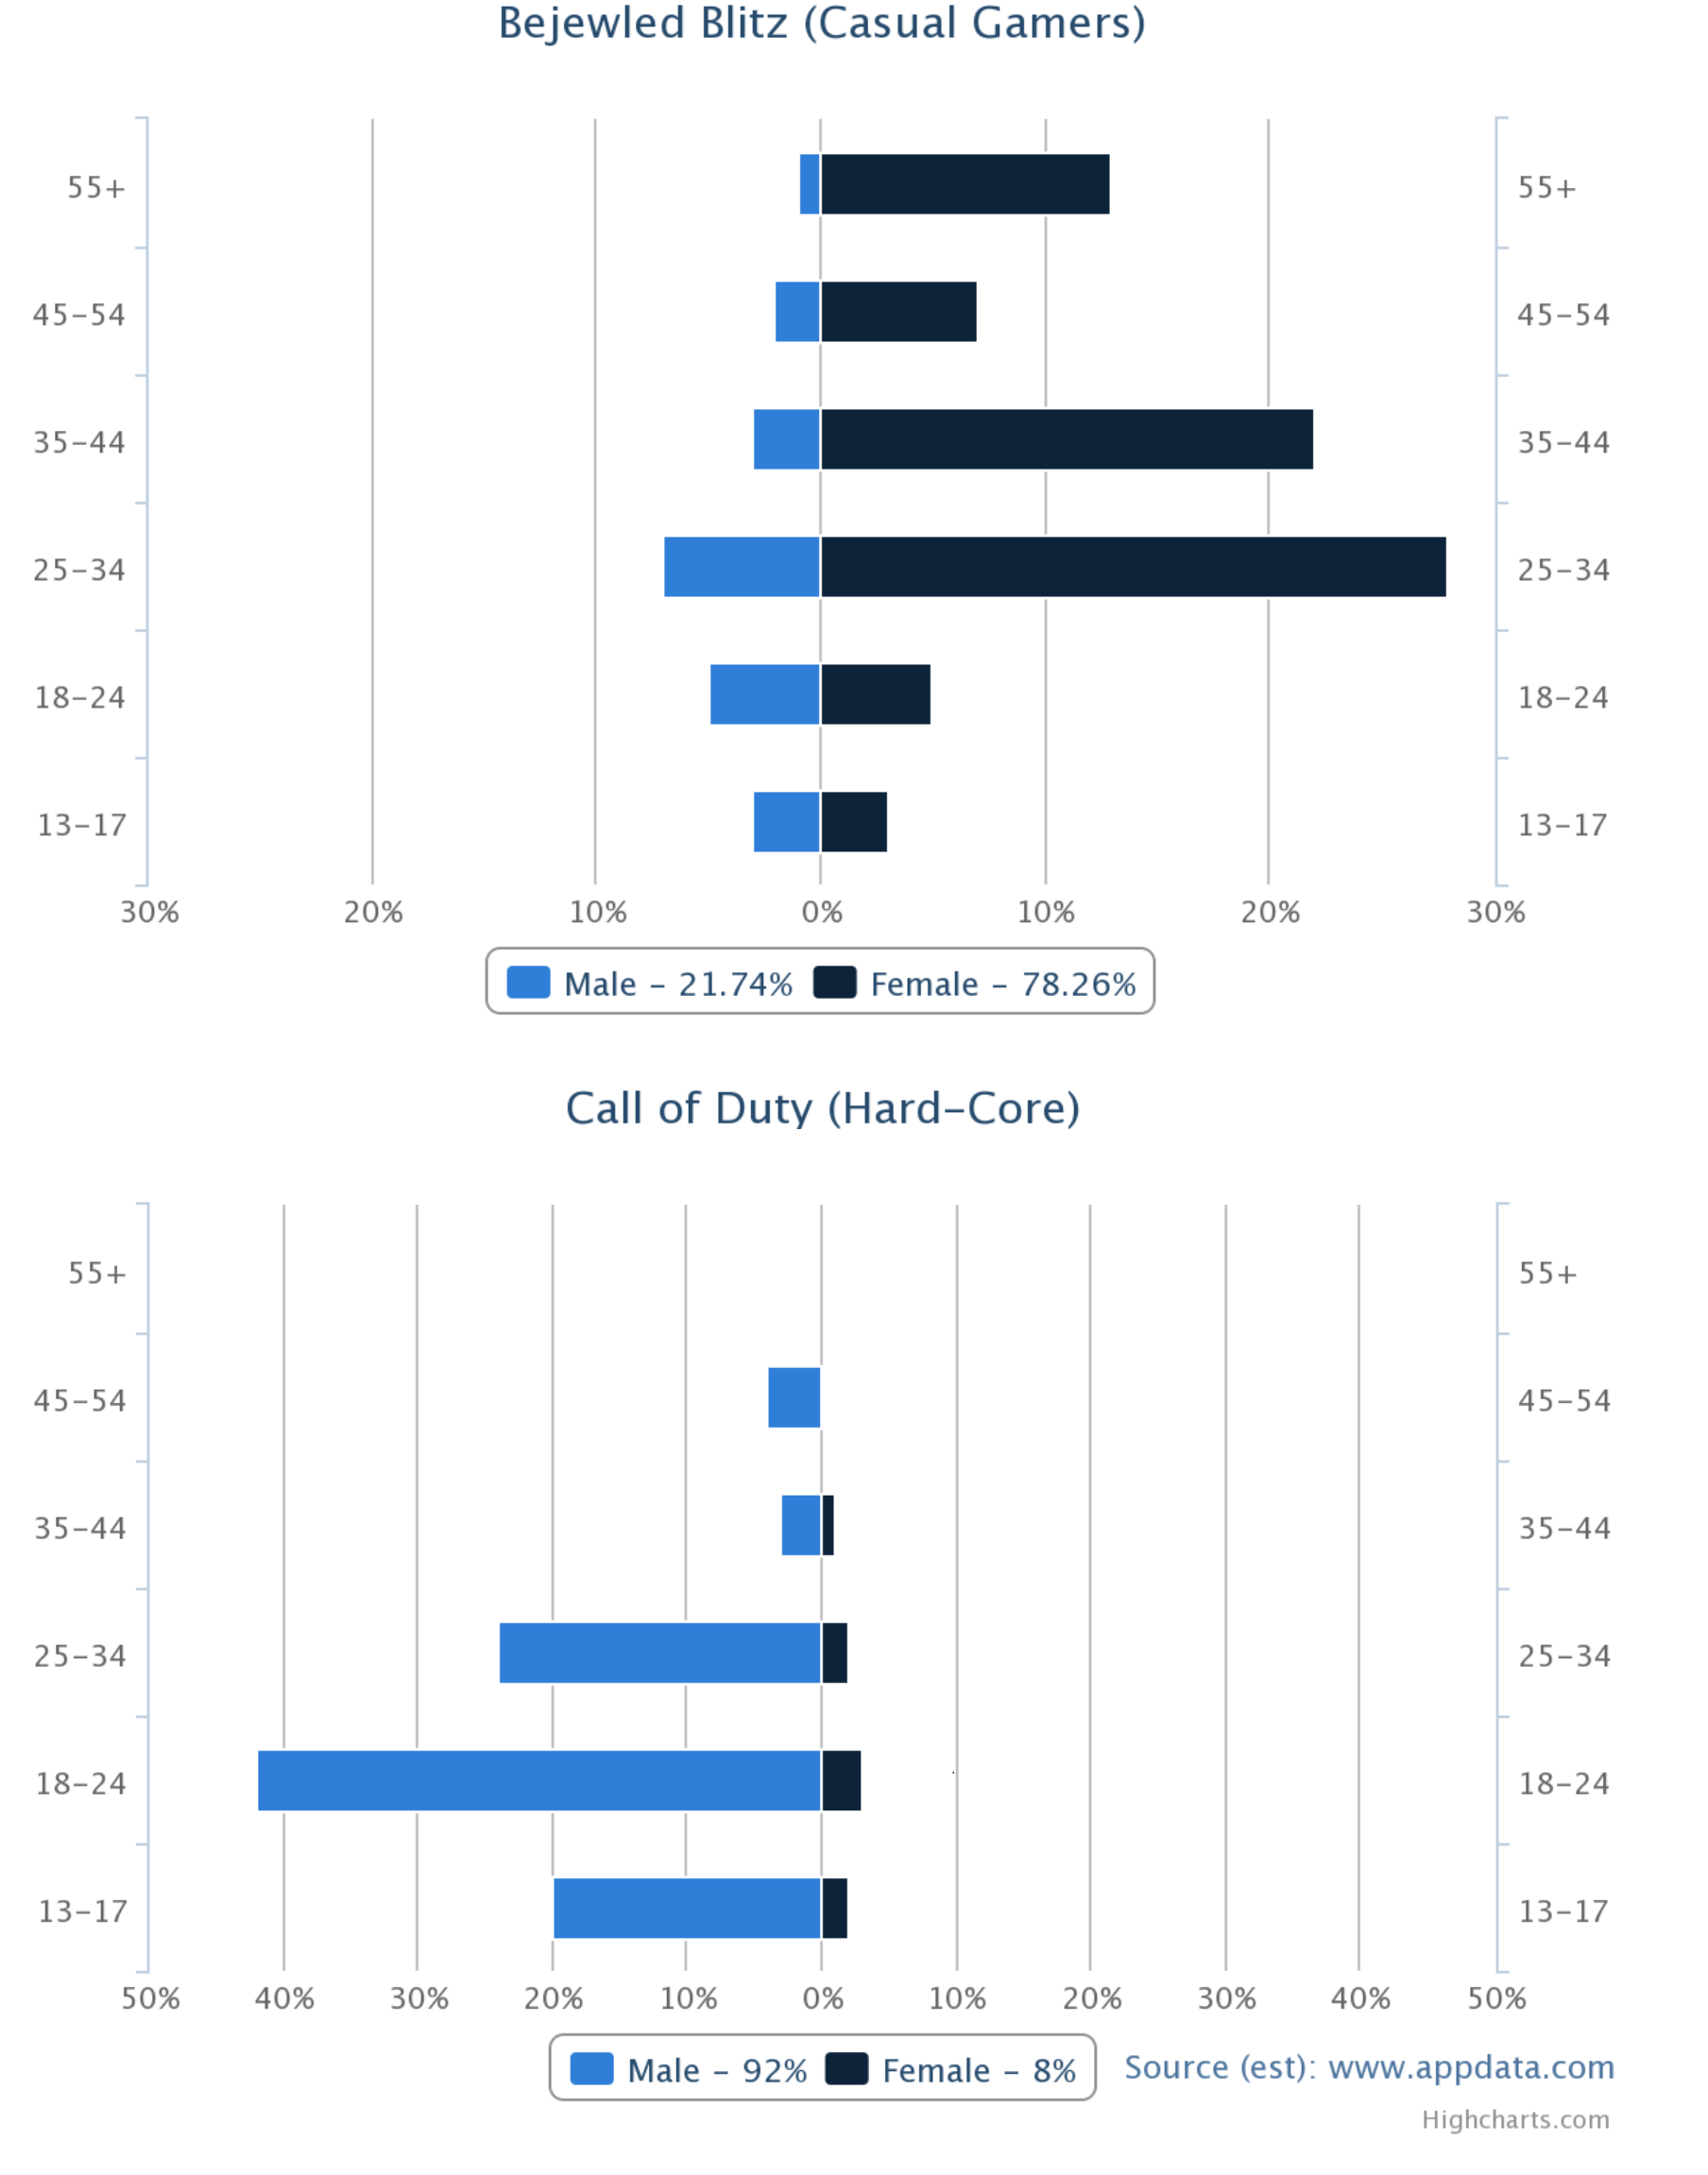
\includegraphics[width=\textwidth,keepaspectratio]{StatsGaming}
					\caption{Casual and Hard-core Game Audiences}		
				\end{center}
			\end{figure}
			
	While the audience of the Hard-core game is primarily male, the audience of the Casual game is primarily female. Gaming in general has a strongly rooted stereotype that it is oriented towards boys and men. However, the data indicates that this is not always the case, and while some games (like Call of Duty) target towards a male market and audience, gaming itself is enjoyed by everyone. \\
			
	As a final example, consider the breakdown by gender of the new up and coming sector of computer science: wearable technology. Wearable technology has only recently began growing as its own subfield of computer science. It aims to bring its customers a fashionable alternative to everyday accessories that are enhanced with technology.\footnote{More information on these figures and statistics can be found in Appendix B and C.}
	
		\begin{figure}[H]
			\begin{center}
				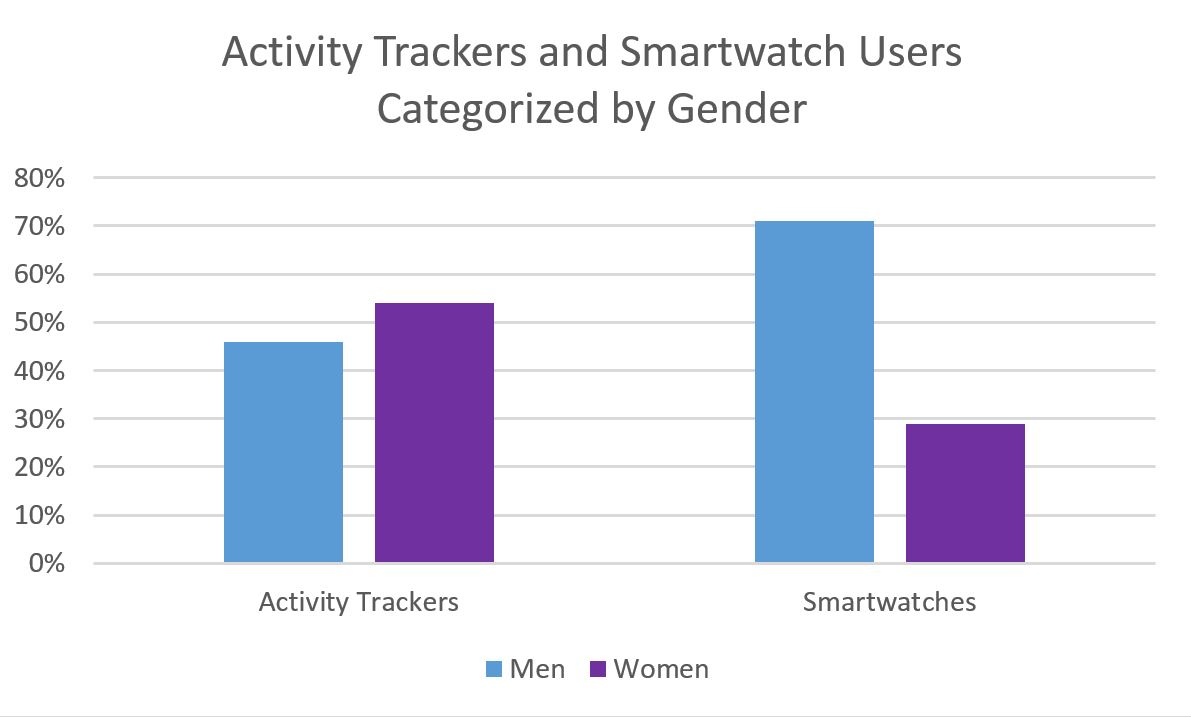
\includegraphics[]{StatsWear}
				\caption{Wearable Technology Users Categorized by Gender}
			\end{center}
		\end{figure}
	 
	 It is important to note, with this example, that women make up the majority of consumers for the activity trackers, while they make up the minority of consumers of smart watches. It can be noted that the design for activity trackers is very gender neutral and can be marketed towards both men and women, whilst the design for the majority of smart watches is very masculine, with huge watch faces and bands that are often criticized for not fitting smaller wrists.\\
	 
	 	\begin{figure}[H]
	 		\begin{center}
	 			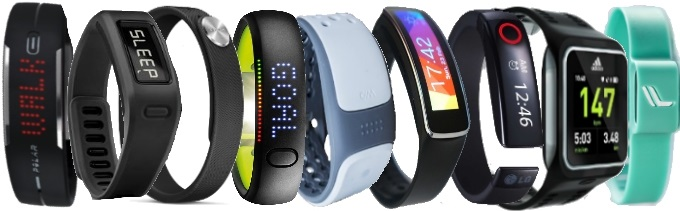
\includegraphics[height = 2in, keepaspectratio]{ActivityTrackers}
	 			\caption{General Design for Activity Trackers}
		 	\end{center}
	 	\end{figure}	
	 	
	 	\begin{figure}[H]
	 		\begin{center}
	 			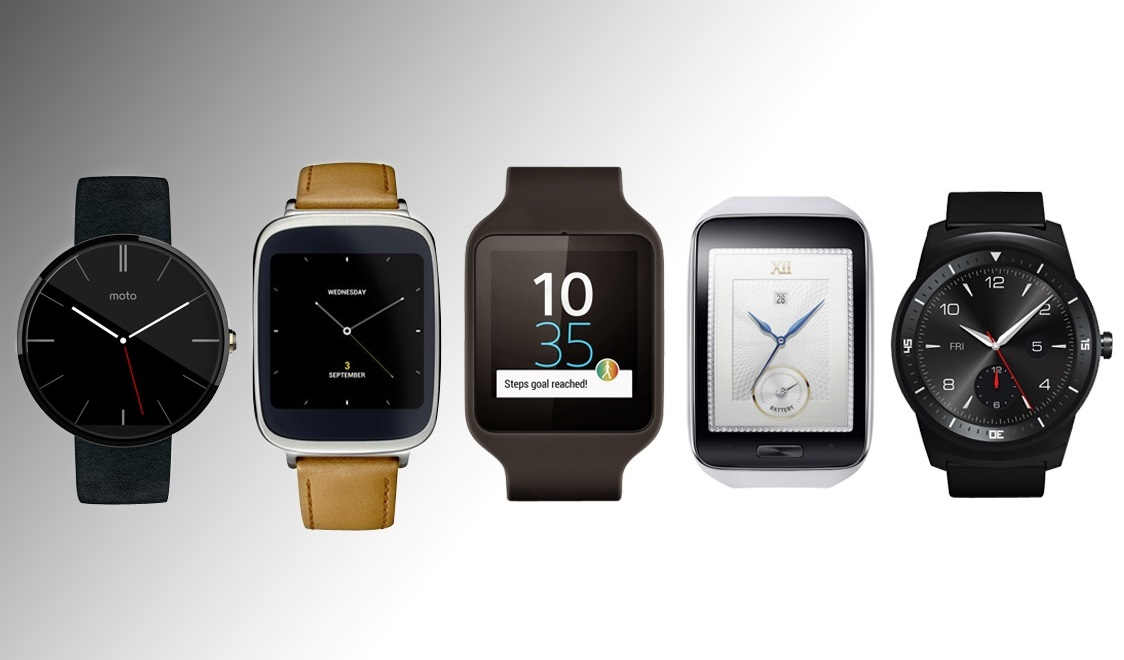
\includegraphics[width = \textwidth, keepaspectratio]{Smartwatch}
	 			\caption{General Design for  Smartwatches}
	 		\end{center}
	 	\end{figure}
	 
	These are just a few examples chosen to fully illustrate how both genders consume and interact with the products made in the technology fields. Yet even though the data indicates that women benefit equally (and in some cases more) from the tools technology provides, few women are learning how to invent, create and design the products they are using. Not only are there not a lot of women in the development teams, but the numbers of women in the workforce and receiving diplomas in computer science are dropping. \\
	
	A recent article on \textit{Fortune} magazine states that In 2013, only 26\% of computing professionals were female — down considerably from 35\% in 1990 and virtually the same as the percentage in 1960\cite{fortune}. These startling numbers are reflected throughout businesses across the entire technology sector. Take for example the data published by Facebook's yearly Diversity report. \\
	
	 	\begin{figure}[H]
	 		\begin{center}
	 			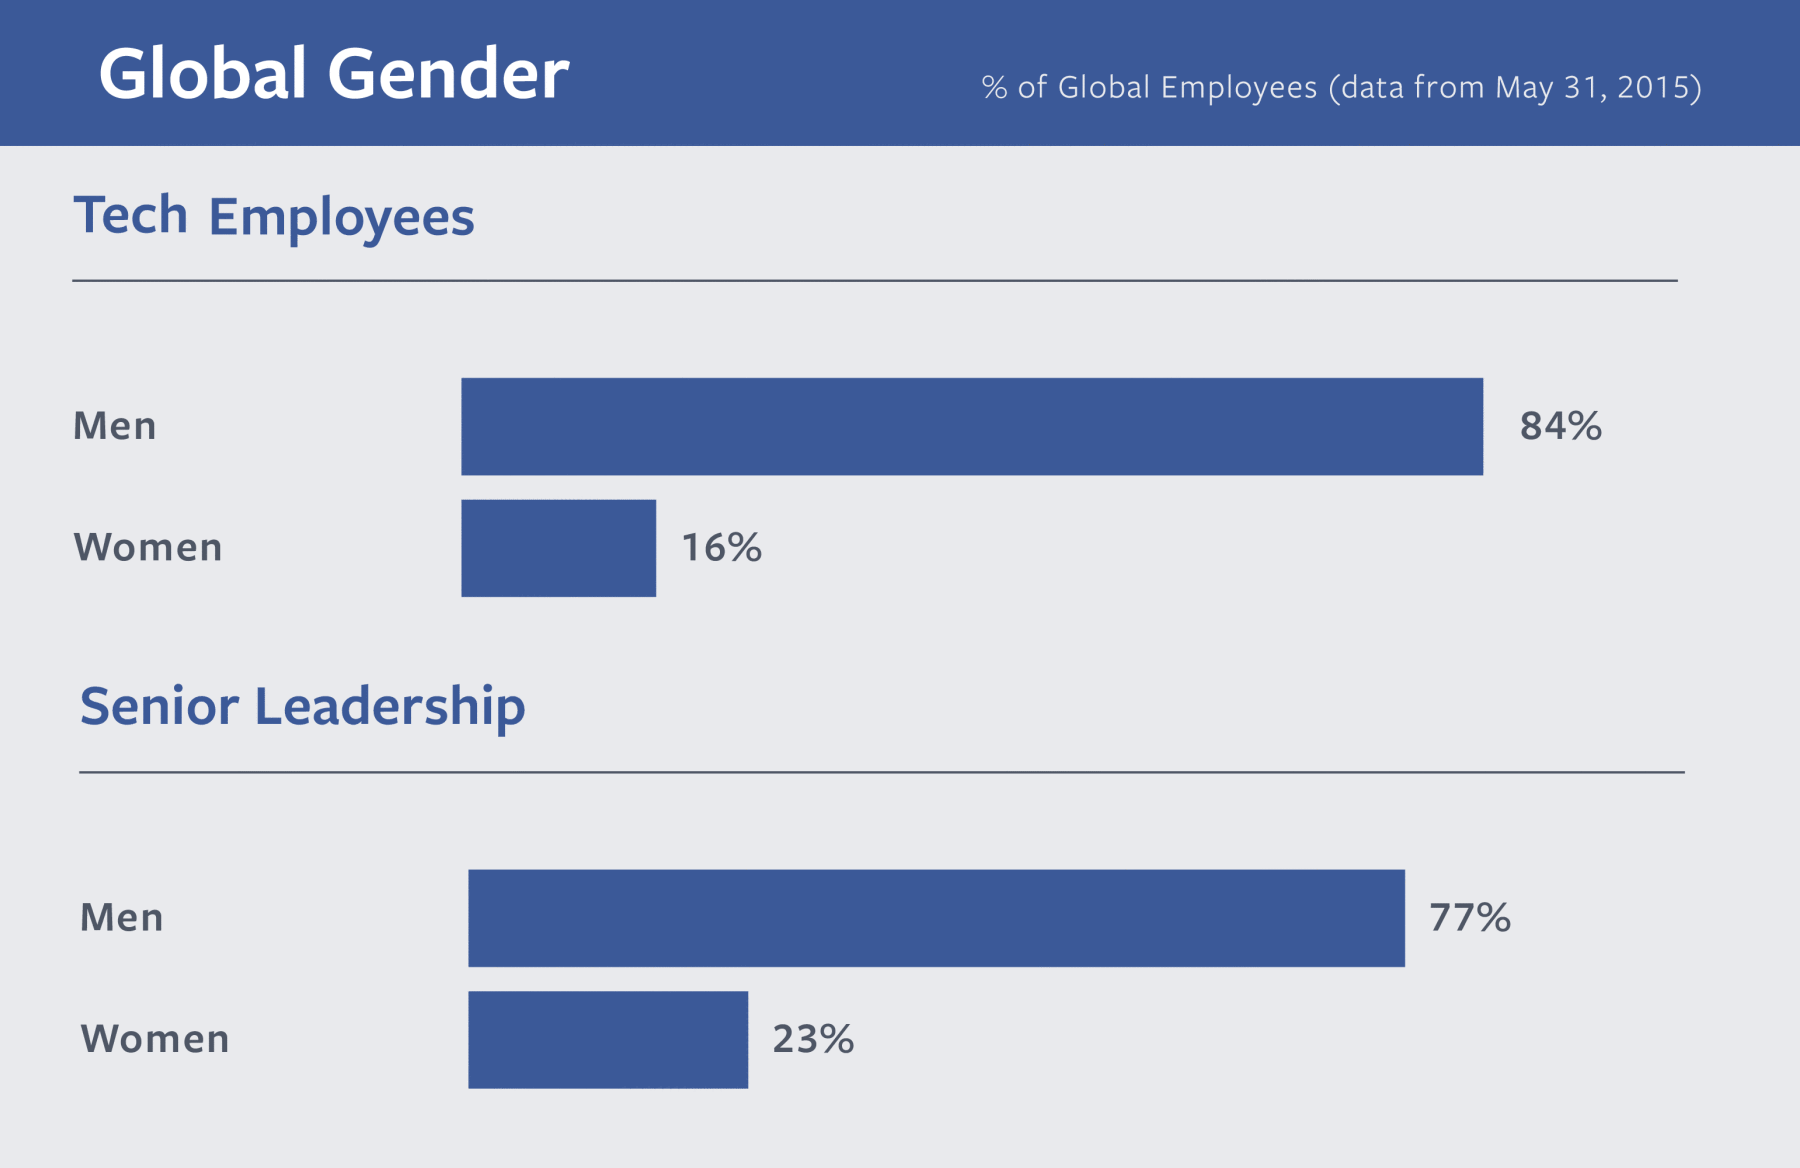
\includegraphics[width = \textwidth, keepaspectratio]{FBDiversityReport}
	 			\caption{Facebook’s Yearly Diversity Data Report}
	 		\end{center}
	 	\end{figure}	
	 	
	Even though, as previously shown, the percentage of female Internet Users  that use Facebook is higher than that of male users\footnote{the previous data showed that 77\% of female Internet users have a Facebook versus 66\% of male Internet users.)} As is shown in the figure, as of 2015 women only make up 16\% of Facebook's tech employees, and hold barely 23\% of senior leadership positions. Similarly, in 2013 Fortune 500 published that only 4\% of Fortune 500 CEO's and 16\% of board directors were female. \\
	
	The data indicates that not only are women already low in numbers in the technology field, but they are also driven out of the field in high numbers.\\

	 	\begin{figure}[H]
	 		\begin{center}
	 			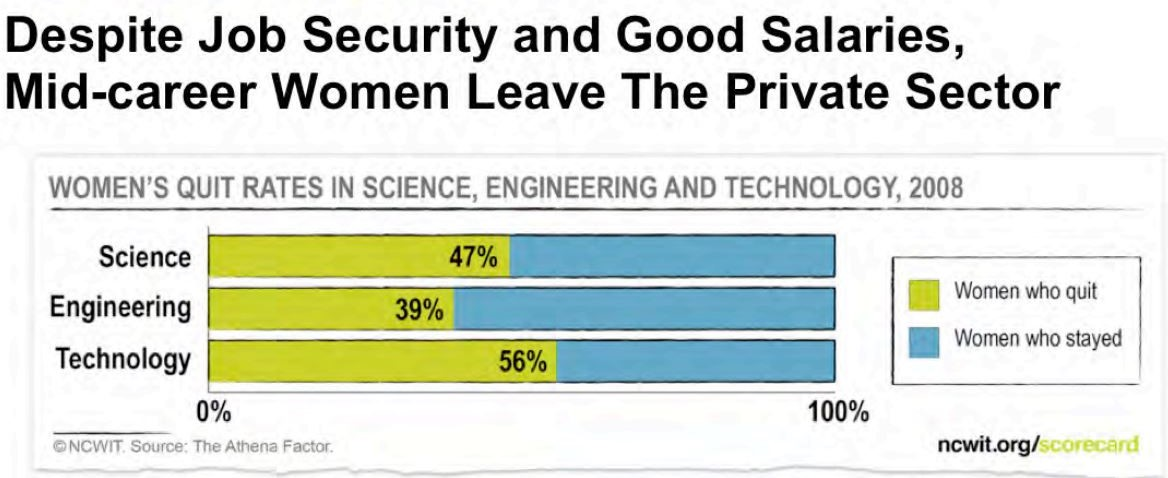
\includegraphics[width = \textwidth, keepaspectratio]{leavingSector}
	 			\caption{Mid-career Women Leave The Private Sector}
	 		\end{center}
	 	\end{figure}	
	
	As can be shown, out of the Science, Engineering, and Technology sectors, the Technology Sector leads the highest quit rate by almost 10\%.\\
	
	Sadly, these numbers are not only shown in a professional setting. The demographics of women receiving PhDs and undergraduate degrees, as well as the number of women interested in Computer Science to begin with reflect these somber statistics as well, especially when compared to the same data towards men. \\

	 	\begin{figure}[H]
	 		\begin{center}
	 			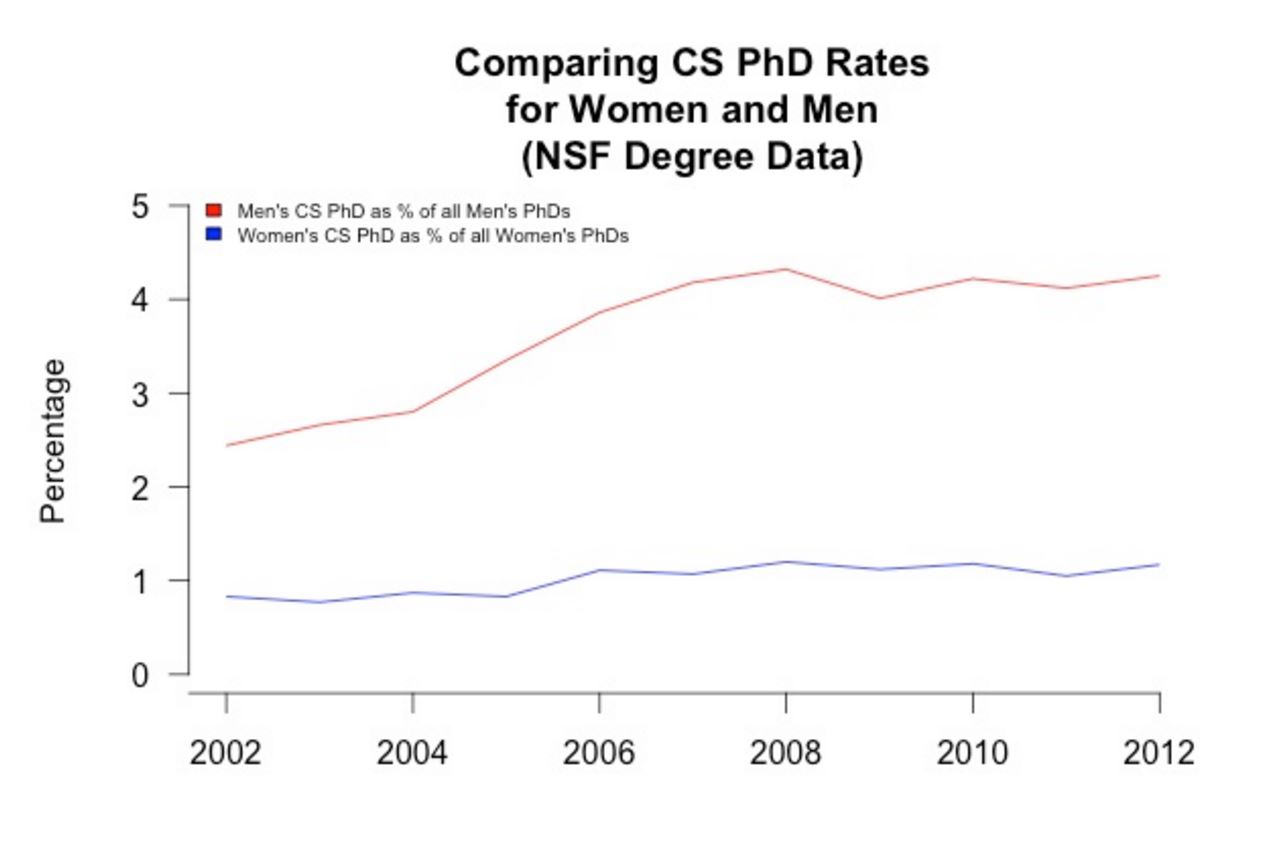
\includegraphics[width = \textwidth, keepaspectratio]{phdRates}
	 			\caption{Comparison of Computer Science PdD Rates for Women and Men}
	 		\end{center}
	 	\end{figure}
	
	 	\begin{figure}[H]
	 		\begin{center}
	 			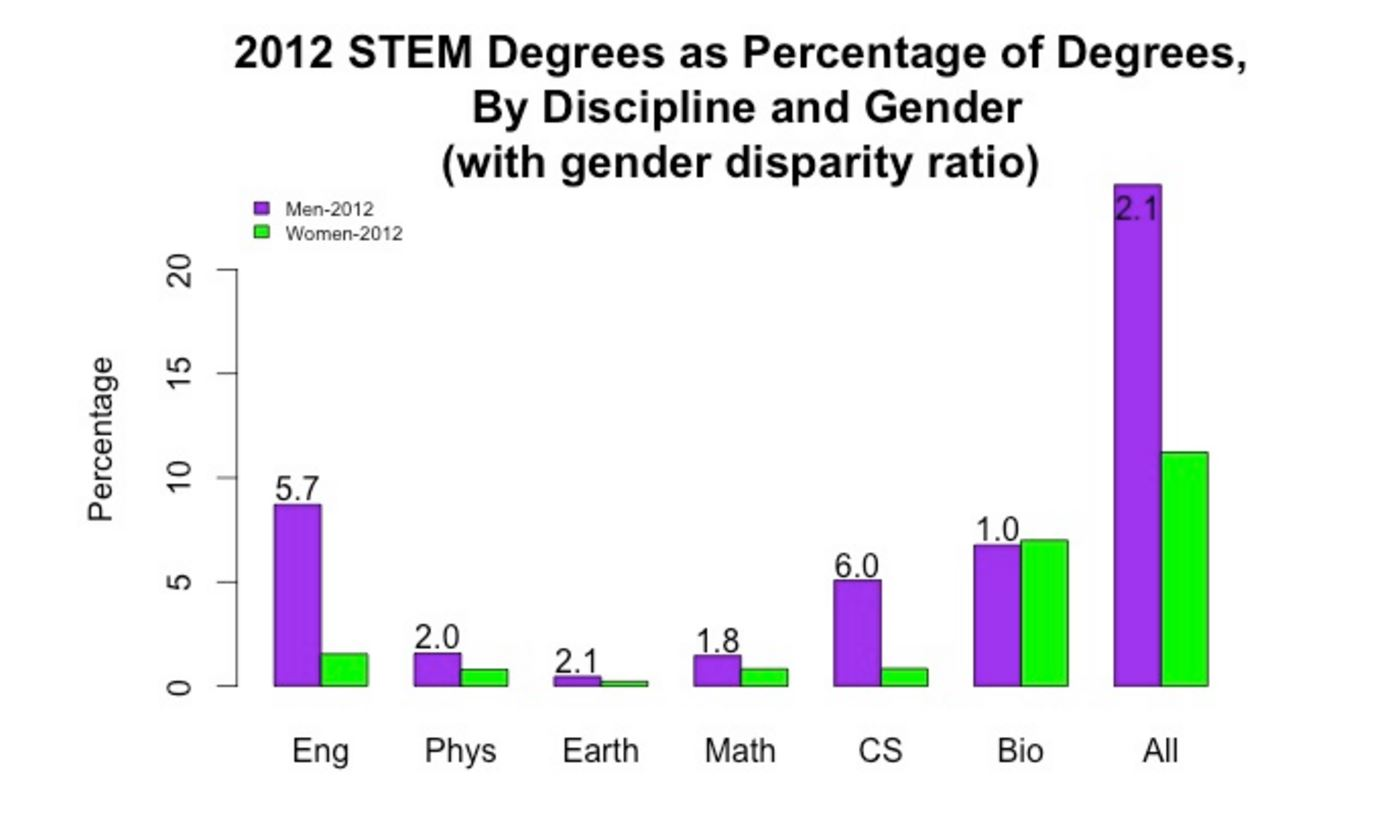
\includegraphics[width = \textwidth, keepaspectratio]{genderDisparity}
	 			\caption{STEM Degrees By Discipline and Gender}
	 		\end{center}
	 	\end{figure}	 	
	 	
	 	\begin{figure}[H]
	 	\begin{center}
	 		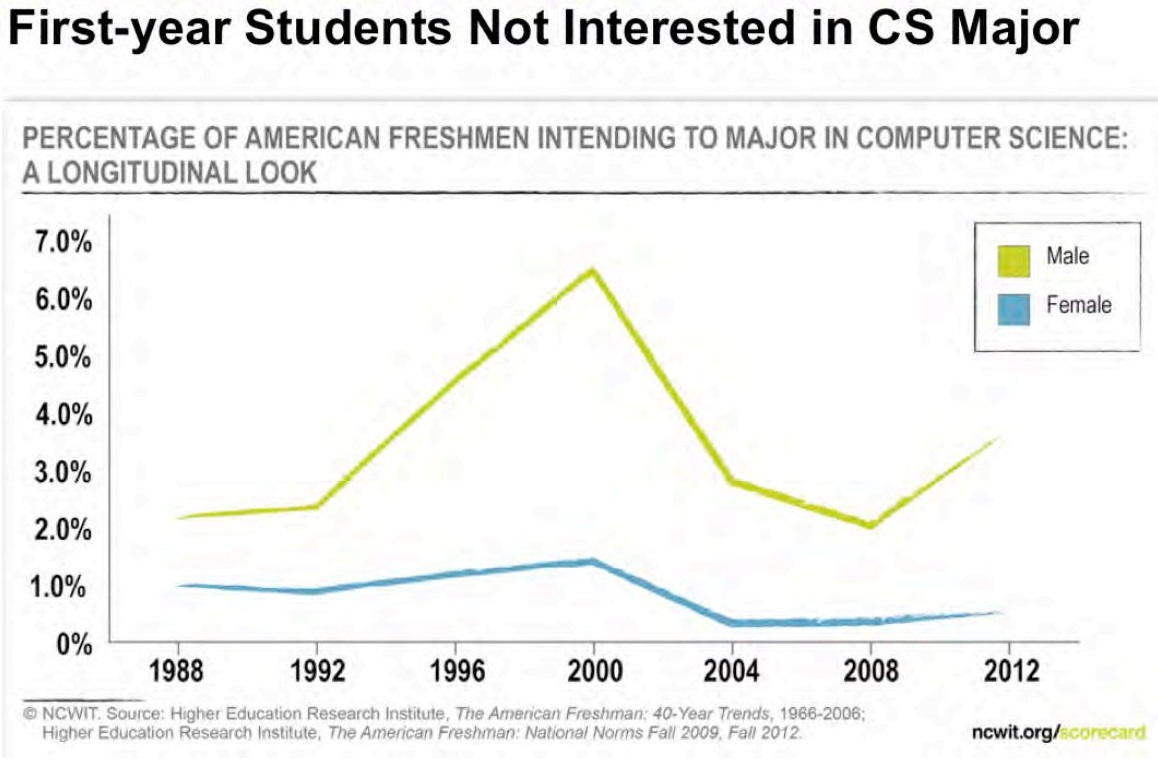
\includegraphics[width = \textwidth, keepaspectratio]{firstYearInterest}
	 		\caption{First-year Students Not Interested in Computer Science Major}
	 	\end{center}
	 \end{figure}	
	
		
	\pagebreak
		

	
	\subsection{Literature Review}
	
	The following literature review will discuss and analyze three different methods that are researched broadly to reduce the gender gap in the Computer Science discipline. By comparing and reflecting upon studies, articles, and books from different sources, this literature review hopes to provide three concrete, approachable, and proved strategies that can be used to attract and retain more women to the field. I would like to note, however, that though these three techniques were found when searching for methods to eradicate the gender gap in the field, they may also be used to diversify the field in general, and attract other types of underrepresented groups in Computer Science, such as people of color or people with disabilities. Also to be noted, this review is not fully intersectional, as it is written with the understanding that all people involved have access to computers and the type of environment where one must work and interact with the computing and programming culture.\\
	
	
	\pagebreak
	
	\textbf{1. Understanding and Talking About the Issues Relevant in the Field}\\
		
		Feeling isolated or ostracized is a common frustration among many involved in the technology field. This feeling of inadequacy can be extremely detrimental not only to a person's performance, whether in the classroom or in the workforce, but also to that person's confidence and self-image. Consequently, this factor is one of the greatest influences that will convince anyone to quit in computer science. Among the many studies focusing on the reasons women in particular are not retained in technology, feeling isolated and unwelcomed is a common thread. Isolation has an impressive power to persuade people to leave the field. \\
		
		Unfortunately, due to the nature of the feeling of isolation, it is hardly ever talked about. So even though there could be many people together who each have developed their own complex impostor syndrome, the needed conversation that would show them they belong is muted. It is hard to talk about feeling ostracized with those that may contribute to that feeling unknowingly. \\
		
		The importance of having conversation, in some form or another, about the adversities that one faces in their personal path in technology cannot be stressed enough. While sharing and listening to multiple experiences, someone who may have been feeling isolated or low in confidence, may be able to realize that those feelings of oppression were not, as they may have believed, self-induced but were actually the unwelcomed results of external factors like implicit bias or wrongful cultural pressures. Additionally, having an honest and open conversation about the experiences and adversities that are faced can help prepare and teach others what to expect, how to handle a problem should one arise, and steps to prevent uncomfortable or discouraging situations. \\
		
		In the study, \textit{Factors that Affect the Physical Science Career Interest of Female Students}, Hazari explores five common hypothesis used to encourage female students to pursue careers in the physical sciences. Of the five hypothesis explored, one had a particularly strong positive effect: discussing the underrepresentation of women in physics class. As the report explains, reflection on stereotypes and underrepresentation issues in the physical sciences, may have lead to greater self-realization for the students and may have shown an effect on their choice of a physical science career. These explicit personal discussions regarding any issues faced in pursuing the sciences helped the students realize that any feelings of inadequacy or discomfort they might have stemmed from external norms and pressures rather than from their capabilities, interests, or values. As the report explains, the importance of the students' self-reflection was fostered by interventions that directly counteracted with these students' stereotypic beliefs, and affirmed their personal values more broadly. This consequently resulted in increased engagement, grit, and confidence. In a closing statement, Hazari concludes "Perhaps engaging in discussions around underrepresentation affords more opportunities for female students' self-realization because the act of discussing may incorporate their perspectives, rather than being inherently teacher centered, and help to affirm their belonging."\cite{hazari}\\
		
		Equally as important as having these conversations is the location where they are occurring. Due to the complexities of having a conversation that can put so many in such a vulnerable position, the importance of a safe space cannot be stressed enough. According to the article \textit{Diversity training in graduate school: An exploratory evaluation of the Safe Zone project}, a safe zone provides an opportunity for people to talk, learn, and ask questions in a non-judgmental, safe, and educational environment. Thus, having a safe zone provides an environment where everyone feels comfortable enough to speak and even more so to listen is key to having these impactful conversations. The article emphasizes that in order to be supportive and aware of different identities, perspectives, and experiences in an ever-diversifying society, we must pursue (and provide) opportunities to learn about these topics from individuals -particularly ones that are stigmatized, marginalized, and largely silenced\cite{safezone}. \\
		
		While it would suffice to have the conversations on their own, they would be much more influential if they were to occur in a location where everyone involved felt comfortable and safe. Whether this safe space was a classroom with a closed door, a meeting surrounding a meal, or a mentor's office, as long as everybody feels comfortable enough listen and speak, the safe space is created.\\
	
		\pagebreak
		
	\textbf{2. Changing the Image: Combating Stereotypes and Stereotype Threat}\\
	
%		\begin{quotation}PG's, Starcraft, etc. Instead, I prefer Call of Duty and sports games. I lift weights and play basketball. I have pretty high "EQ" and am emotionally awar
%				\singlespacing
%				\textit{"How well would a non-stereotypical computer programmer fit in in a programming environment? I don't play Re and sensitive of others' feelings (high empathy, I guess you could say.) I enjoy interacting with people on a one-to-one basis. I do like sci-fi though! \\\singlespacing I know stereotypes are just generalizations, but I would supposed there is a high degree of validity in them. I'd really like to work in an environment where I can fit in, instead of feeling left out because I'm not "geeky" enough."}
%		\end{quotation}
%		
%		
%		\begin{quotation}
%			\singlespacing
%				\textit{ You will fit in fine. Totally stereotypical computer programmers are rare at this point. I am actually not sure they were ever common.}\cite{quora}
%		\end{quotation}


		\begin{figure}[H]
			\begin{center}
				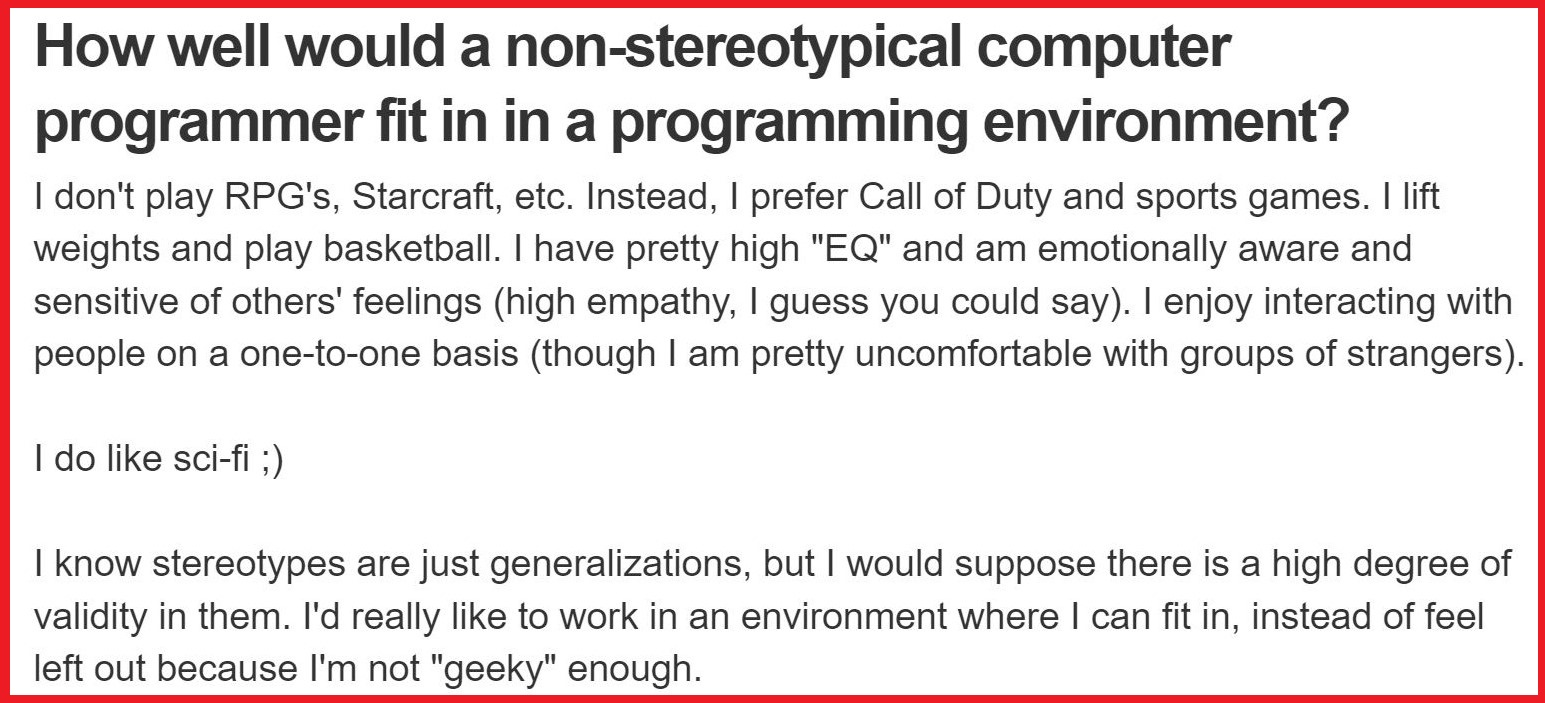
\includegraphics[]{quora}
				\caption{Programmer Stereotype Entry in Question \& Answer Website Quora}
			\end{center}
		\end{figure}
		
		Unfortunately for the Computer Science industry, programmers have earned a rather misleading stereotype that they are distinctively white men with only one type of personality: misunderstood computer geniuses that compensate for their lack of social skills with an incredible ability to compute. The personification of computers themselves. This stereotype origins from years of pop culture, wrongful marketing, and a cultural obsession with transforming successful computer scientists to fit this image. For example, in the movie \textit{Steve Jobs} by director Danny Boyle, Jobs is portrayed as prickly, demanding and unforgiving. He is repeatedly shown to be uncaring and unsentimental when it comes to other people. Throughout the entire movie, Jobs clashes with nearly everyone, as he cares little over whether he is liked or not\cite{stevejobs}. In another example perpetuating this stereotype, note the way Alan Turing, the so-called father of computers, is displayed in the movie \textit{The Imitation Game}, by director Morten Tyldum. The film strongly implies that Alan is a genius somewhat inept at socializing: his character doesn’t understand jokes, takes common expressions literally, and seems indifferent to the suffering and annoyance he causes in others\cite{imitation} all while single-handedly ending World War II with his computational skills. This image contrasts highly with the description of Turing in his biography: a man with a keen sense of humor, close friends, and an inclination to mock bureaucracy and red-tape who was a pivotal role in cracking intercepted coded messages that enabled the Allies to defeat the Nazis, but achieved this by working closely and successfully with a team of highly capable programmers.\\
		
		This powerful, negative, and incorrect stereotype of a programmer (and of women involved in the computing business) is partially responsible for the lack of diversity in the field. As one considers which field they will enter (or continue in) they reflect upon their performance in it. Thus, as Margolis explains in her book \textit{Unlocking the Clubhouse: Women in Computing}, each student's self-evaluation becomes a critical part of his or her sense of belonging in computer science, and the myopically obsessed computer whiz types have become the reference group- a frame of reference for each student's self-evaluation and attitude formation. An exceptionally high level of obsession and expertise has become the expected norm and has raised the bar for the level of knowledge, interest, and expertise identified with computer science majors. \textit{Unlocking the Clubhouse} reports a study performed in Carnegie Mellon University where researchers conducted interviews with more than 100 computer science students. Margolis explains that in the study, seeing most of their male peers as totally absorbed in computing, produced a fear that "I don't seem to love it as much as the men, and therefore I don't belong," to lurk in many women's doubts\cite{margolis}.	Margolis also found that while the stereotype of the computer science student as someone who is myopically focused on computing is rejected by many male and female students, women reported more distress and were more affected by the perceived difference between themselves and their peers. As many as one fifth of the women interviewed questioned whether they belonged in computer science because they felt they do not share the same intensity in focus and interest that they saw in their male peers\cite{margolis}.\\
				
		The glorification of the myopically obsessed computer programmer can also force a second stereotype where anyone who does not fit this image is not a competent or successful computer scientist. This consequently produces a phenomenon called stereotype threat, a situational predicament where people feel themselves to be at risk of confirming stereotypes about their social group. There are many studies that show that awareness of negative stereotypes associated with how a person identifies inhibits their performance, confidence, and feelings of belonging. One such study, of women experiencing stereotype threat in mathematics, \textit{Stereotype Threat Reduces Motivation to Improve Effects of Stereotype Threat and Feedback on Women’s Intentions to Improve Mathematical Ability}, showed that a negative image of a female mathematician impaired women's performance and buffered their self-esteem from negative feedback (therefore causing a reduction to their motivation to improve their mathematical abilities)\cite{fogliati}. The author of the study stresses the importance of identity-safe environments to reduce the impacts of stereotype threat. For example, avoiding the display of any media (such as posters, books, pictures or videos) that imply a certain group of people will over or under perform or any mention that one group may do better. \\
		 
		The singular and obsessive interest in computed is often assumed to be the road to success in computing, ultimately shaping the assumptions of who will succeed and who "belongs" in the discipline. However, according to Margolis' study, over half of the students interviewed linked their interest in computing to other arenas, describing their passion for the field as "computing with purpose." In fact, many students mentioned contextual concerns and links to social concerns as their greatest reason to study Computer Science. For example, connecting programming to social work, health, or environmental issues. From these results, Margolis claimed that a critical part of attracting and retaining different people to the discipline is providing multiple ways to "be in" computing. Concern for friends, family, and a programmers hobbies should not come at the cost of success in Computer Science, but rather be an integral and important component of achievement. \\
		
		Computer Science is often associated with number-crunching and quantitative skills. In order to bring more diversity to the discipline, we shouldn't have to fit students and professionals to this image, but rather invoke a cultural and curricular revolution to the way that the field is presented so that different perspectives and values are respected within the discipline. \\
		
		Additionally, there are many proven ways to combat stereotype threat. According to \textit{Reducingstereotypethreat.org}, performance issues caused by stereotype threat can be reduced or eliminated by several means. The article describes 7 different approaches that work to overcome the adversity: reframing the task, deemphasizing threated social identities, encouraging self-affirmation, emphasizing high standards with the assurance about having the capability to meet them, providing role models, providing external explanations for difficulty, and emphasizing an incremental view of intelligence\cite{threat}. On a more individual level, \textit{Serve.org} published an article researching and confirming an old hypothesis that reflecting on the other values in a person's live beyond school or work can help them reduce the impact of any stereotype threat they may experience within themselves\cite{believe}.\\
	 	
	 	\pagebreak
	 					
	\textbf{3. Role Models Used to Introduce and Retain Women in Computer Science}\\
	
		The following section will explore the different impacts  of a role model as a mean to introduce and retain more women in Computer Science. Surprisingly, the studies researched and discussed here showed very different results for this approach when used to attract women than when used to retain them.  \\
		
		The first study, \textit{Enduring Influence of Stereotypical Computer Science Role Models on Women’s Academic Aspirations}\cite{typerolemodels} focused on the impact of specific role models upon undergraduate women who were not Computer Science majors. The study was founded upon the role model presenting a lecture with the students and then having a 2 minute interaction with each student. The study aimed to discover whether these role models could increase the students' interest in Computer Science. What the researches found was that regardless of gender, if the role model presented embodied the Computer Science stereotype in appearance they had an immediate and negative  effect on the women's interest in the field. In fact, if the role model embodied the stereotype, the women's scene of belonging in computer science decreased, especially following the 2 minute interaction.\\
		
		This article showed that being exposed to stereotypic role models could have a negative impact on student's interest in computer science. However, it is hypothesized that being exposed to female role models could counter stereotypes in students, and help them realize their potential to engage in belong in the science communities. In the study mentioned before, \textit{Factors that Affect the Physical Science Career Interest of Female Students}, Hazari also explored whether this hypothesis was true. Surprisingly, the research yielded null results with respect to female role modeling. They explain that while it is a common belief that role modeling is necessary for attracting females, focusing on role models didn't effectively encourage the women simply because  seeing a woman in science didn't connect with the subjects. The authors explained that reading an article about a brilliant woman scientist, or hearing stories about a seemingly flawless programmer felt unrelatable, and made the career seem out of reach. \footnote{On the other hand, this study also found that having a supportive teacher and mentor of any gender made a big difference in the students' decision. Researchers found that relationships developed within the context of the discipline were critically important, regardless of the gender of those relationships. A large number of the women studied reported that a person, not necessarily female, influenced their choice of career. Thus, mentors that had built a positive relationship and implemented well-meaning practices were found to be much more influential than role models for students deciding their careers.}\\
		
		While these studies showed that the exposure to role models didn't seem to peak women's interest in the field, other studies prove that strong and relatable role models can be very effective in \textit{retaining} women in the field. Once they are interested, role modes have been shown to be an effective means to continue interest and passion. \\
		
		For example, the study \textit{Undergraduate Women in Science and Engineering: Effects of Faculty, Fields, and Institutions Over Time} found that the percentage of women among undergraduate science majors was associated with and positively correlated with the percentage of women among the faculty in their fields. In other words, exposure to female role models in the institution they were studying increased the number of female college students who were enrolled in that institution. A final study, \textit{The effect of a role model project upon the attitudes of ninth-grade science students} showed that intervention using female role models was found to improve the attitudes of ninth grade students and that it directly correlated with the students' attitudes towards their field. The study found that female role models in the science classroom was an effective way to maintain students' attitudes towards the topic.\\
		
		The research towards the effect and impact of female role models was very surprising. While female role models made a powerful impact on students that were already interested in the field, they weren't as effective towards introducing and attracting students to the topic. Not as surprising, however, was the role of the mentor, which in both cases showed to have a strong relation towards a student's choice in their career. \\
		
	\pagebreak
	
	\subsection{Research Conclusion}
	
	
	As was shown in the research, women utilize and benefit from the services of technology as much as (and in some cases more than) men. Unfortunately, the inventors, designers, and creators of these technologies are not as gender diverse as the users and benefactors of them. Even though there is a shortage of employees in the field, the pay is impressive, and the opportunities for career growth are often emphasized, talented women who could work in this discipline are discouraged and disaffected from pursuing computing careers. At the most basic and individual level, women who have the necessary talent and inclination who do not engage with the Computer Science sector are missing the educational and economic opportunities that are so abundant in the field. On a less individual level, non-diverse teams are less likely to produce products that meet the needs of  gender-diverse audience. The people behind any technological service define the parameters of that product, since the technical decisions behind that product will be based on the experiences, opinions, and judgments of the team behind it. Hence, when women are underrepresented in the production teams, the resulting product will be made to match the needs and desires of men (even if the targeted audience included women as well.) The design of any product is a reflection of the team behind it. A wildly discussed example of this is gaming, which often reflects on the fears, anxieties and desires of boys and men. However, there are many other historical and shocking examples of when a male majority in the production team created a very male-skewed and biased object. Early voice-recognition systems did not recognize the higher pitches of a female voice (literally silencing women) a problem that still persists today, as many car voice command systems do not register the voices of female drivers. The first models of face-recognition software for videos would not register a female face, as the bone structure, voice pitch, and facial hair was often different than the prototypes used in the development process. In an example combining the gender disparities in engineering and technology, the original airbags were made to protect an unbelted average-sized male in a 35 mph crash, thus most of the people killed by airbags were children and women (this was rectified \textit{8 years} later in 1998 by the Transportation Equity Act)\cite{airbag}. Perhaps one of the most current and pronounced examples is wearable technology, the fusion of fashion and technology. If wearables are designed by exclusively (or majorly) men, then even if the intended audience is the general population, the resulting product will have been produced with men in mind. Smart watches are often criticized for this due to their large, masculine watch faces and bands intended for larger wrists. Wearable technology in particular caters to products intimate to their consumer's style and individual fashion preferences. These products need to be optimized for people of not only all genders, but also all skin colors, abilities, body types and ages. This emphasized diversity in the target audience requires an equally diverse development team that can provide input from a broad range of perspectives and experiences. Increasing the number of women in the field wouldn't just benefit the women excluded from it now, but it would help destroy some of the uncovered gender bias that has distorted major technological products and services. \\
	
	
	Diversity must be a characteristic of the development teams who are reshaping the world, if the reshaped world is to fit our diverse lives. Unfortunately, many people do not feel as if the belong in the Computer Science world. This impostor syndrome stems (pun intended) from many different factors, such as an exclusive and hurtful image, a misunderstanding of the field, the everlasting impact of stereotype threat, lack of role models, and lack of mentors. Fortunately, there exist many proven and successful strategies to battle these dangerous influences, such as role model and mentor intervention, awareness of the issues prevalent, open communication, community support, and stereotype threat awareness. \\
	
	In a digitally developing world, working, studying, and understanding technology and computing is a privilege. The lack of diversity in the computing world isn't due to a lack of interest, but due to a harmful and segregating environment. Welcoming more diversity to the computing world will ensure that the products and services created are reflective of the audiences and users benefiting from them. Not only that, but when institutions, like schools and professions, become more inclusive, everyone benefits (not just the newly included groups.) One of my favorite examples of this is the curb ramps at the end of sidewalks; intended to help people on wheelchairs, they've become assets that help everyone, such as people with strollers, suitcases, or bikes.  \\
	\pagebreak
	
	\section{Taking Action}
	
	A lot of institutions recognize the impact having a large imbalance in diversity can cause, and strive to provide structural support and encouragement to prevent homogeneity among its employees, students, or members. They recognize that we cannot simply \textit{wait} for more women to suddenly become interested in computing and create a pipelining influx of new women employers and students, but rather that there are many different ways to provide encouragement and motivation in order to retain and introduce more diversity to the field.\\
	
	In 2015, the Anita Borg Institute published a list of the top companies for women technologists, listing Bank of New York (BNY) Mellon as the top company supporting diversity. BNY Mellon illustrates many different types of institutional support towards diversity, such as management awareness and training on unconscious bias, holding many employee resource groups such as Prisim, which strives to promote an open and supportive environment for all LGBT employees, WIN (Women's Initiative Network) which aides the professional development and advancement of BNY Mellon's women employees, or IMPACT which helps recruit and retain multicultural employees.  BNY Mellon also holds many kinds of special events and programs that help promote diversity and inclusiveness.\\ 
	
	As an example of an academic institution that has largely contributed to the diversification of technology and computing, take private research university Carnegie Mellon. \textit{Women@SCS}, or Women at School of Computer Science, is an advisory committee consisting of undergraduate and graduate students, faculty, and alumni of the Carnegie Mellon School of Computing that have collaborated throughout to years to construct an inclusive and supportive evironment for the students. Perhaps the group is best illustrated through their website, found at \textit{women.cs.cmu.edu}.\\
	
			\begin{figure}[H]
				\begin{center}
					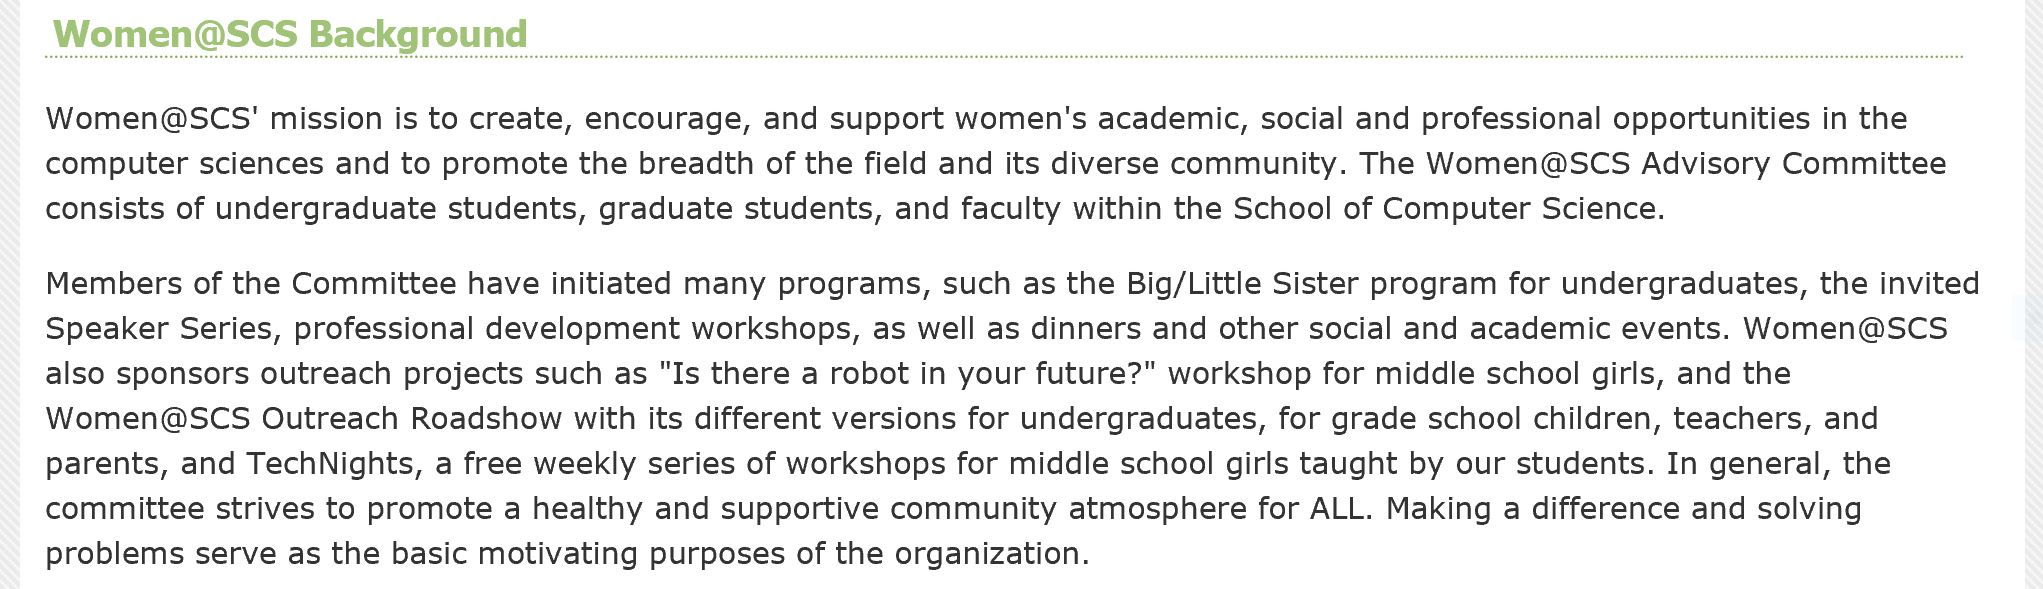
\includegraphics[width=\textwidth,keepaspectratio]{CarnegieMellon}
					\caption{Women@SCS Description}
				\end{center}
			\end{figure}
			
	The website provides plenty of resources and information tailored to women at Carnegie Mellon, such as a calendar showing the upcoming evens such as TechNights, Outreach programs, conferences, or expositions, information about upcoming programs, internships, and visitors, information on mentoring and joining a big sister/little sister program, resources for finding job and research opportunities and career advice and even interviews with Carnegie Mellon alumni and faculty.
	
		
		
		\begin{figure}[H]
			\begin{center}
				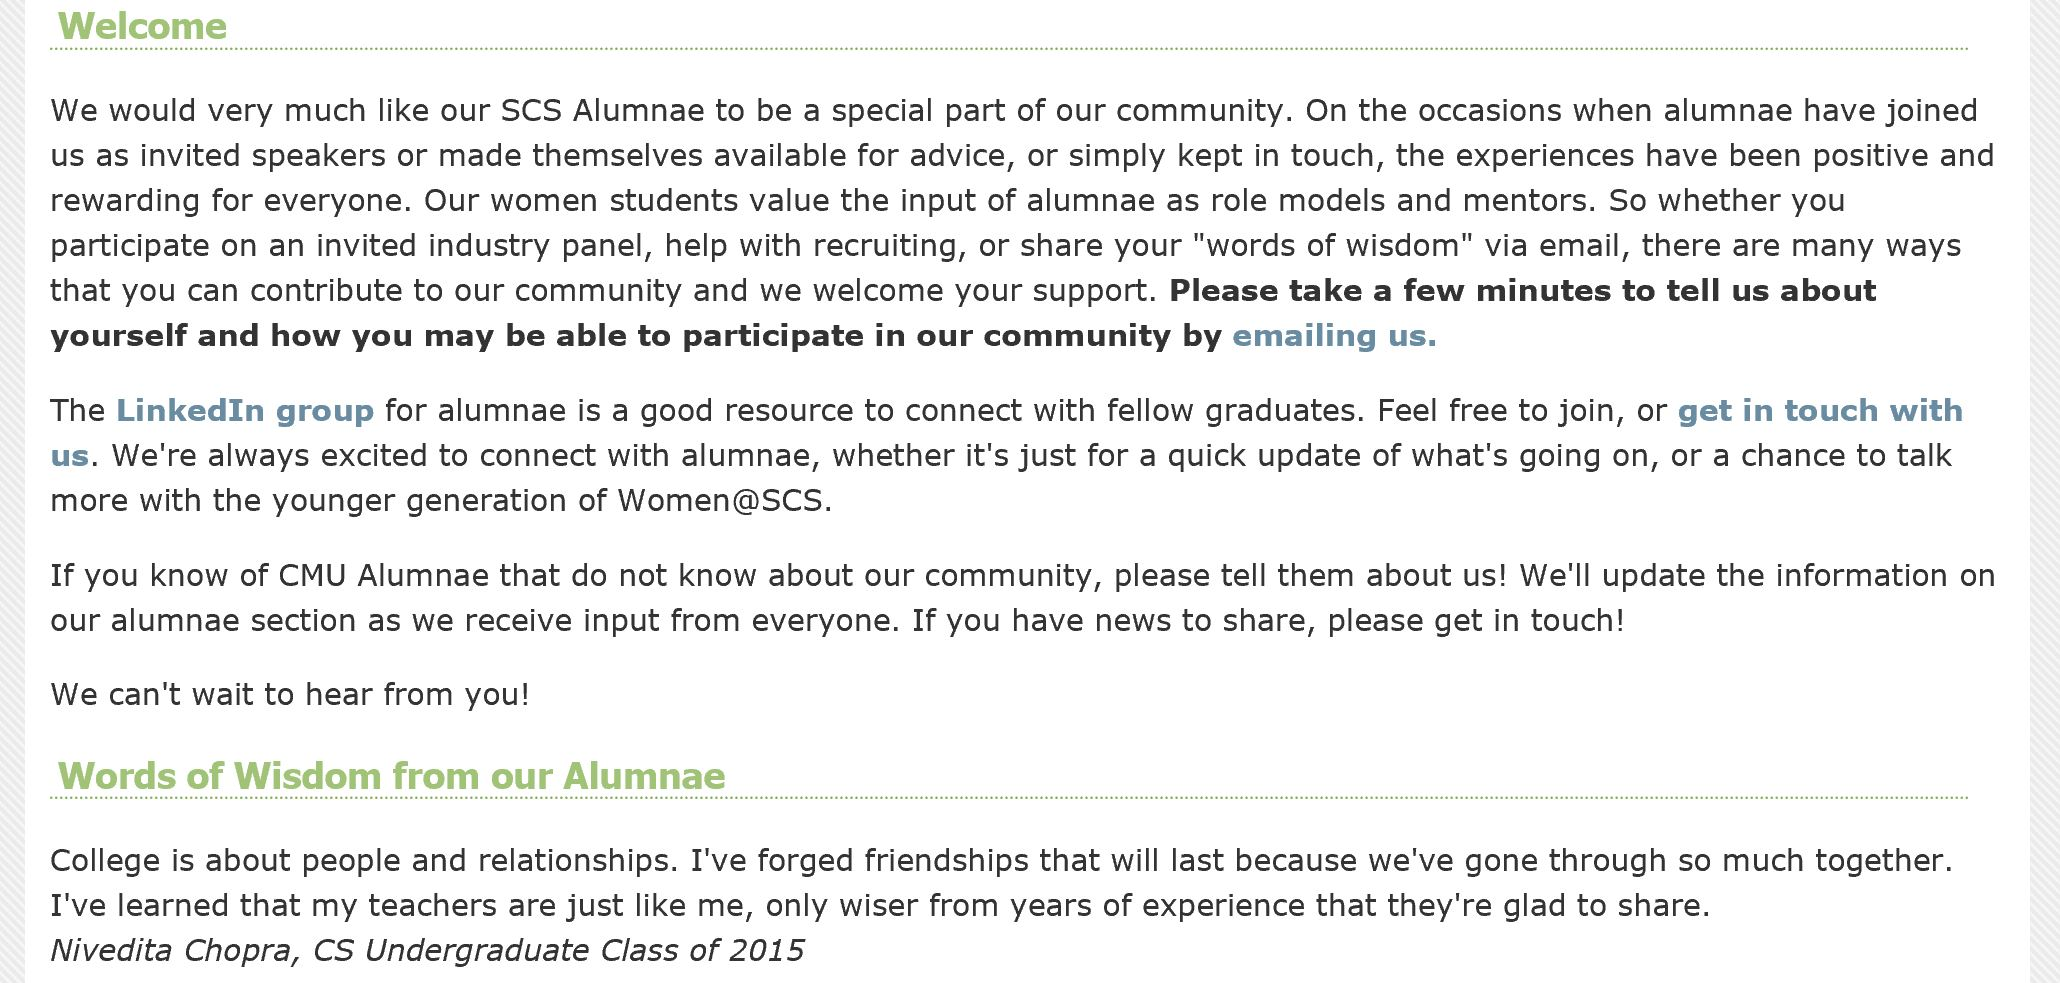
\includegraphics[width=\textwidth,keepaspectratio]{CarnegieAlumni}
				\caption{Interviews With Carnegie Mellon Computer Science Alumni}
			\end{center}
		\end{figure}
		  
	
	As a final example for institutions that encourage diversity in technology, The Office of Science and Technology Policy, in collaboration with the White House Council on Women and Girls. In recognition of the lack of diversity in STEM (Science, Technology, Engineering and Mathematics) the White House published a website, called \textit{The Untold History of Women in Science and Technology} dedicated to sharing the stories of impressive women in the sciences. \\
	
			\begin{figure}[H]
				\begin{center}
					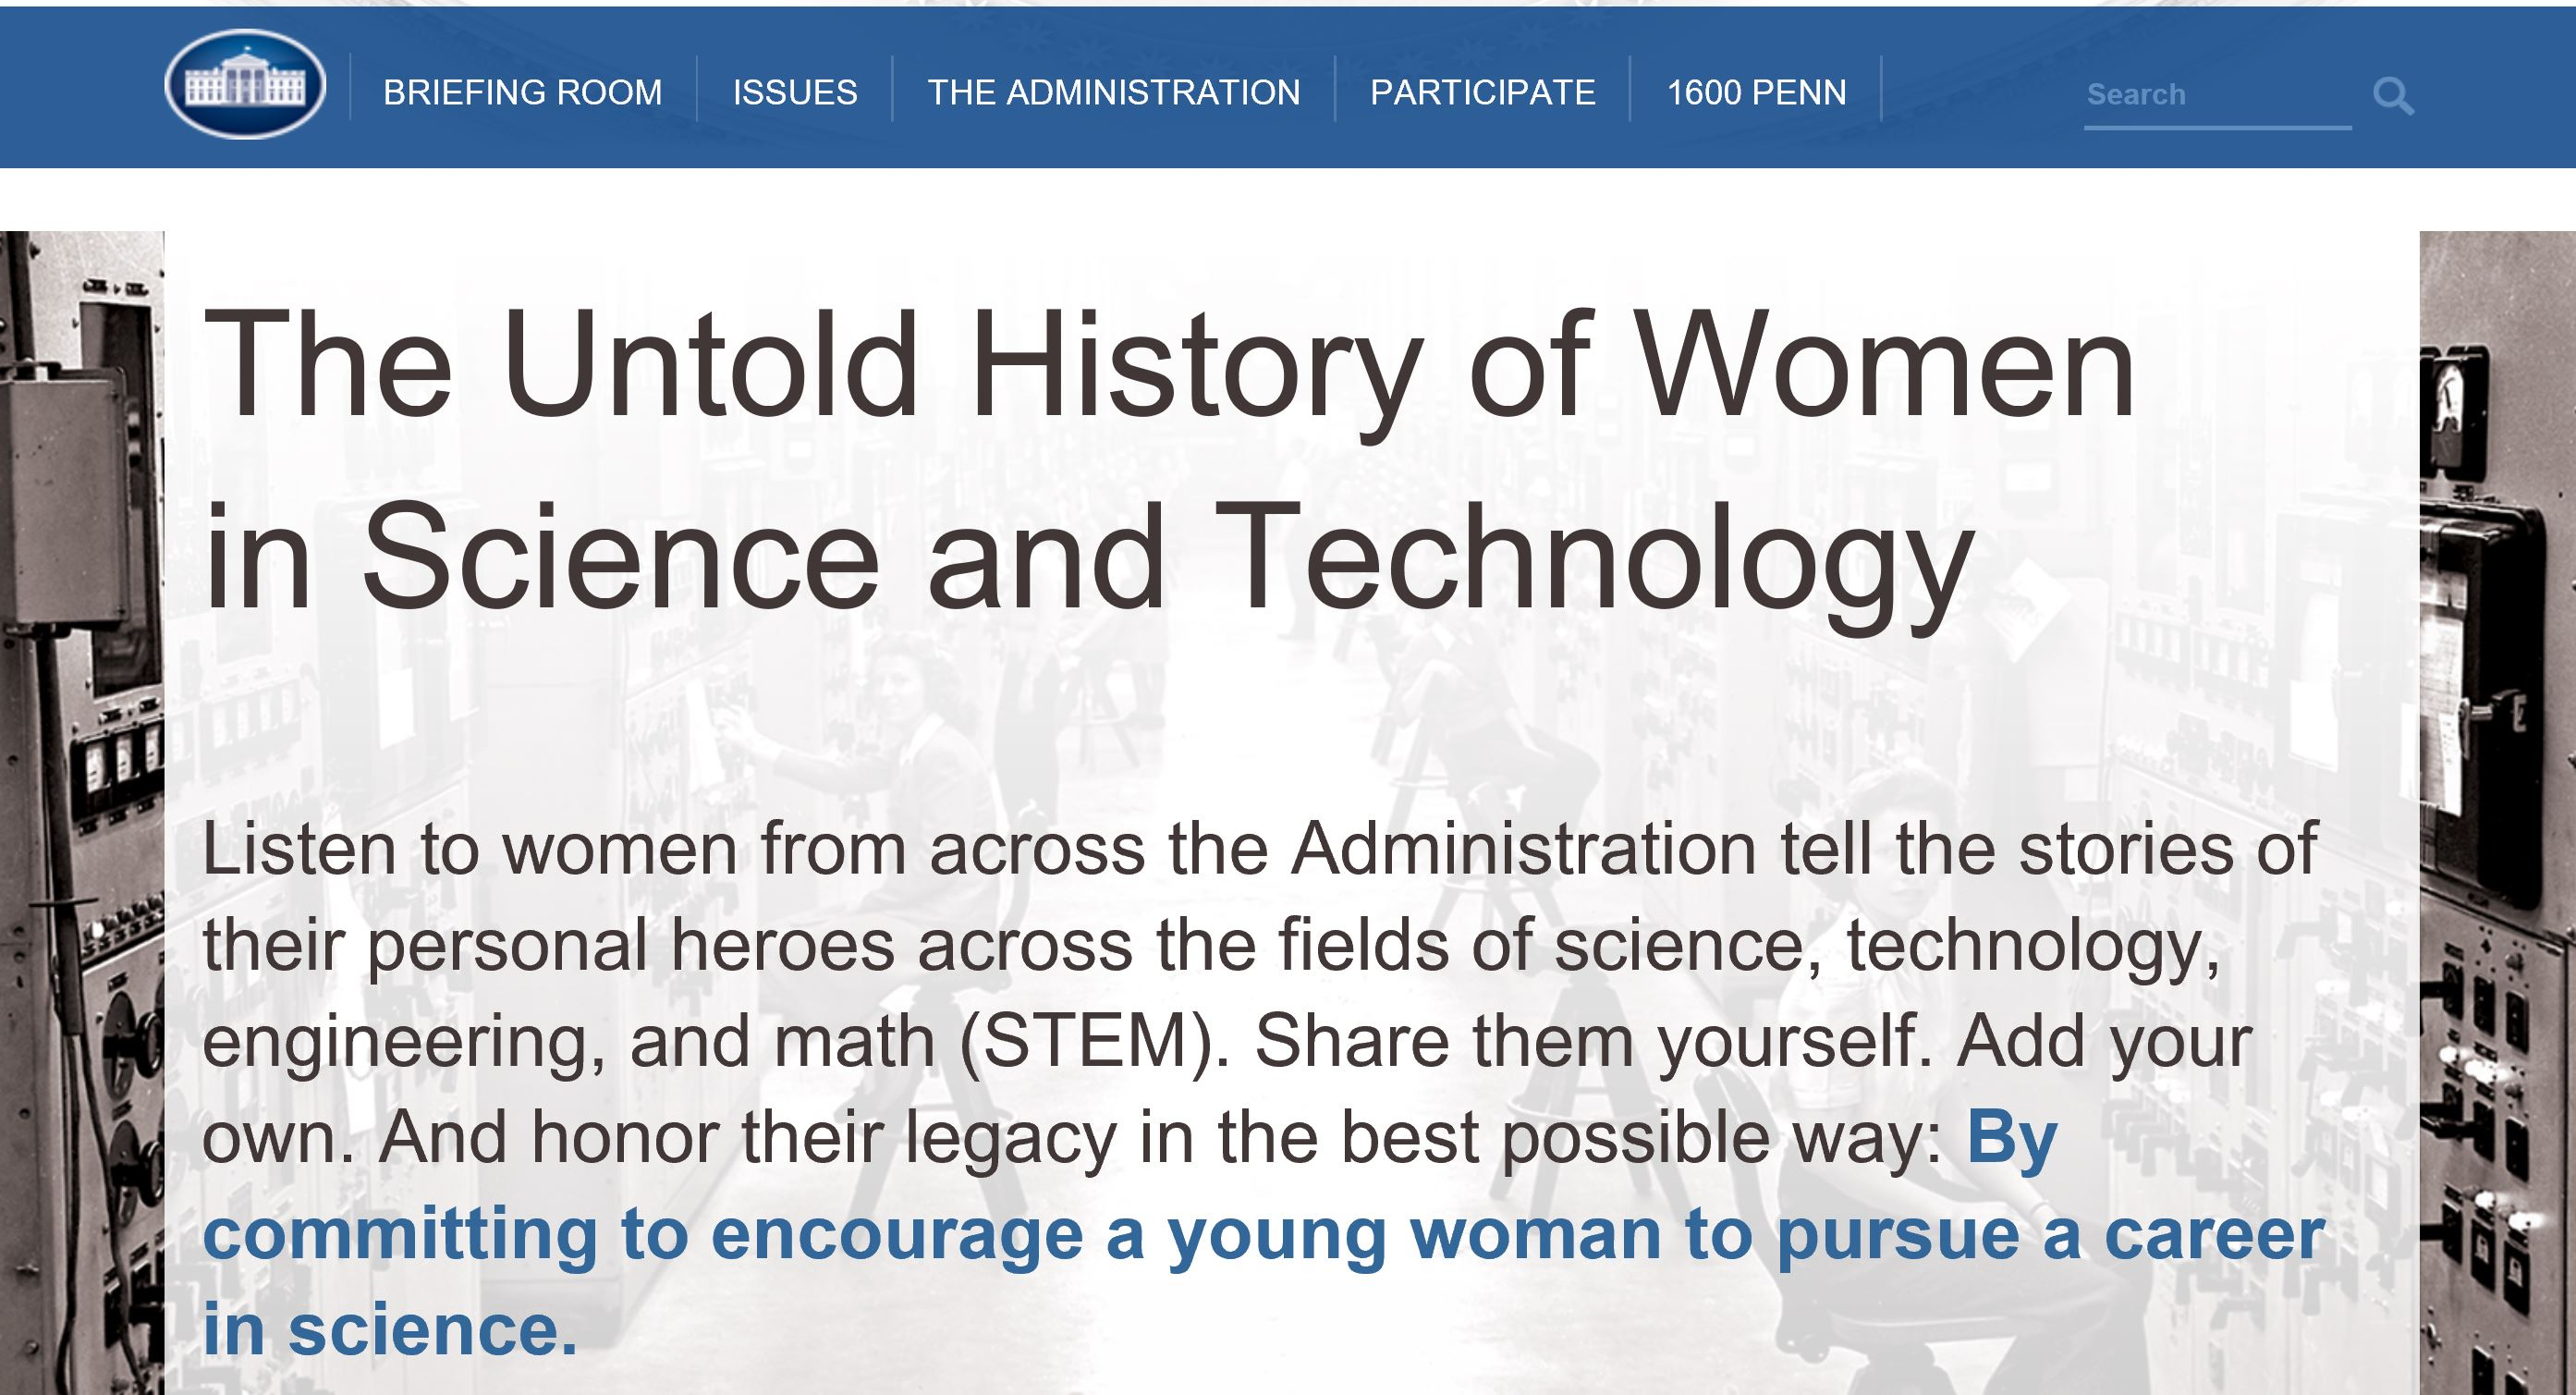
\includegraphics[width=\textwidth,keepaspectratio]{WhiteHouse}
					\caption{Description of White House Website, The Untold Story of Women in Science and Technology}
				\end{center}
			\end{figure}
			
	The website, found at \textit{whitehouse.gov/women-in-stem} shows both a written biography and a sound clip description of impressive women, such as historic Ada Lovelace (considered the first computer programmer and founder of scientific computing) and the ENIAC Programmers (the 6 young women who programmed the first all-electronic computer in World War Two).\\
			
			\begin{figure}[H]
				\begin{center}
					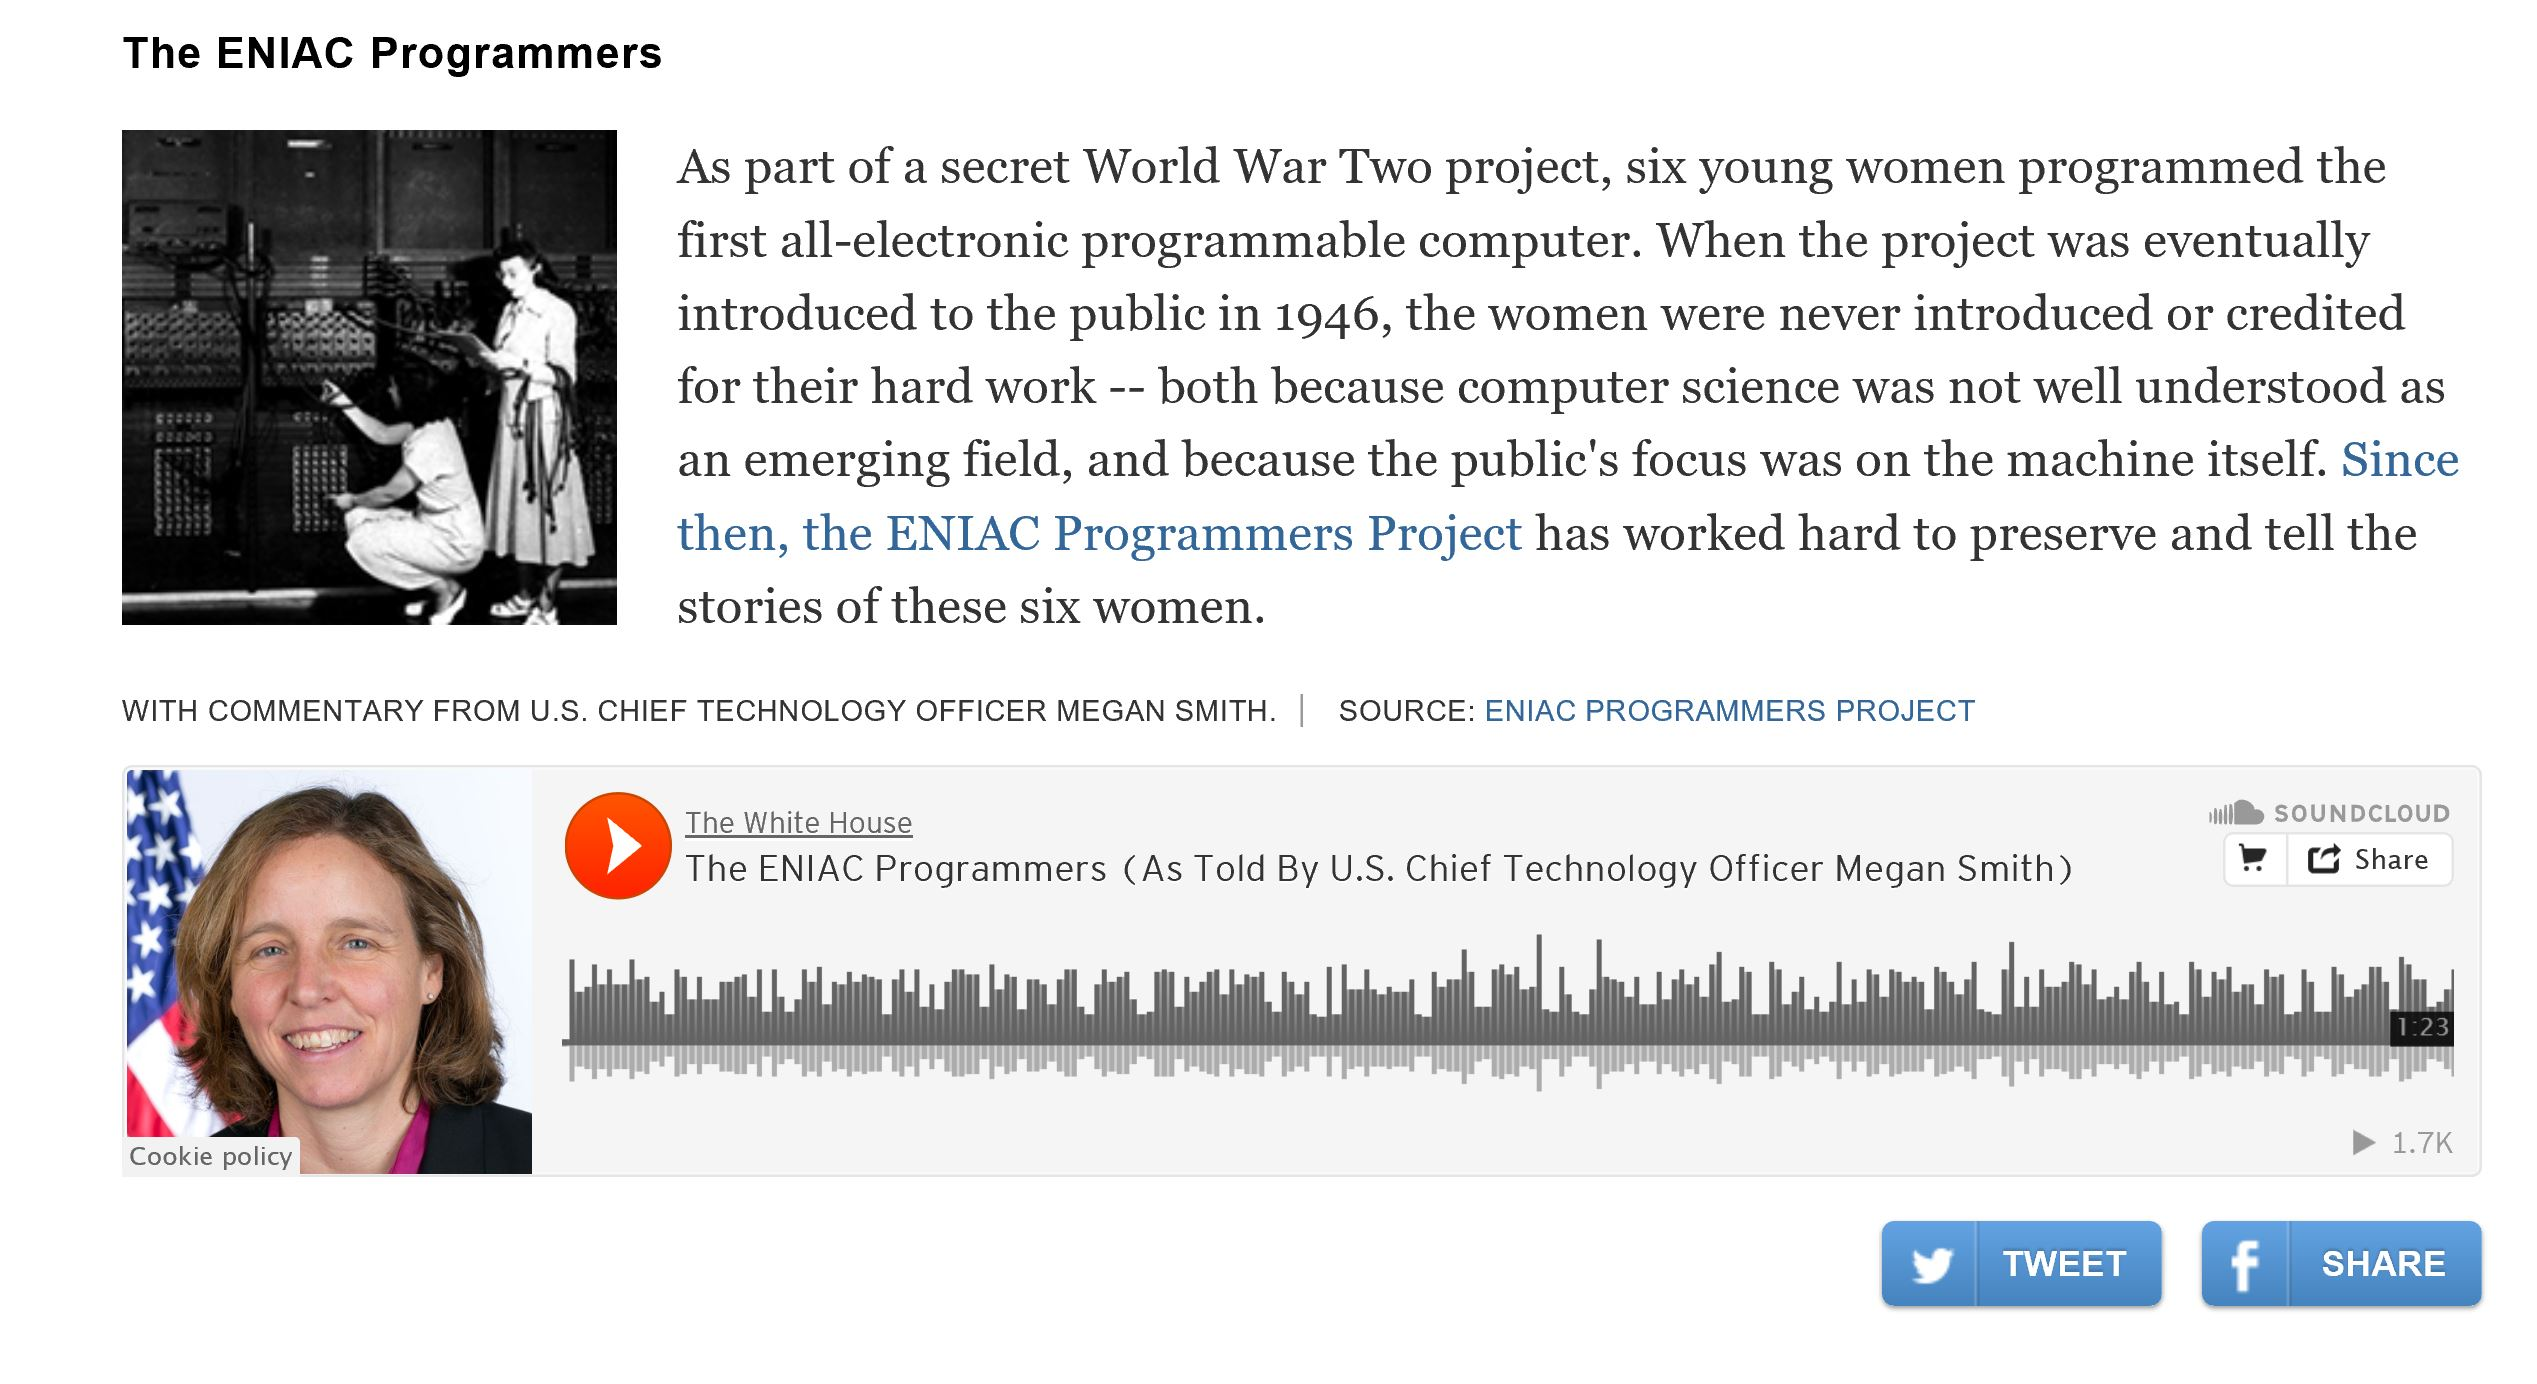
\includegraphics[width=\textwidth,keepaspectratio]{WhiteHouseExample}
					\caption{Example of White House Website Entry}
				\end{center}
			\end{figure}
			
	
	These three examples, and many others like them, illustrate the three strategies mentioned before that can be used to reduce the gender gap: encouraging community and dialog, changing the image of computing (and the stereotypes with it), and providing role models and mentors. In their own unique combination  they use these strategies, among others, to encourage more women to try out computer science and to stay involved. \\
	
	As a second portion to my SIP, I wanted to follow in the footsteps of these leading enterprises, and produce a similar platform for Kalamazoo College. Kalamazoo College offers a couple venues of structure to encourage students in pursuit of their studies, like the Women in STEM lunches, the Women in CS lunches, and the occasional speaker. However, while helpful, these events are strictly occasional. The women in STEM and CS lunches happen once a term or once a year, and in my four years I have only been aware of two speakers addressing the issue:  The 2014 Jennifer Mills Lecture with Eileen Pollack (called \textit{How we can (finally) get more women into STEM fields}) and the 2015 Women in CS Lunch with Kalamazoo College Alumni and Google employee Pan Fayang.\\
	
	The following sections will describe my process and experience building a place at Kalamazoo College whose mission is to make Computer Science more inclusive and diverse. I wanted to follow the examples of structures built before, like those described earlier and others similar. I will be describing what worked, what didn't work, what surprises I found along the way, and the response and feedback received by the community.\\
	\pagebreak
	
	
	%%%%%%%%%%%%%%%%%%%%%%%%% FIRST TRY %%%%%%%%%%%%%%%%%%%%%%%%%%%%%%%%%%%%%%
	
	\subsection{Trial and Error}
    The women in STEM website and the Carnegie Mellon website shared one characteristic that immediately called my attention and attracted me: they showed people in that = community that had accomplished great things and were willing and happy to share their stories. In the White House website, this can clearly be seen, as sharing the stories of accomplished women in STEM is the main purpose of the site. on the Carnegie Mellon website, this is one feature of many, but one that can be seen clearly throughout the site through interviews with the schools faculty and staff, TAs, upperclassmen, graduate students, and alumni. \\
    
    While both the Carnegie Mellon and the White house website show a picture, description, and contact information for the people featured, the stories on the Carnegie website have a special focus that the White House website doesn't mention: they display more than just professional achievements. On this site, you can find stories of facing adversities, anecdotes of self doubt or impostor syndrome, and how each individual interviewed perseveres. Take for example this quote from Carnegie Mellon alumni Lisa Nelson: 
    
    \begin{quotation}
    	\begin{center}
    		\singlespacing
    		\textit{When I told some of the male students not in the Department that I was majoring in Computer Science, they would look at me as if I "took their spot" and would give me unfriendly looks. I started to feel embarrassed to tell people my major and questioned whether I got into this school just because I was a female. I went to see the Freshman Advisor for Computer Science, Jim Roberts, and said, "If I am in here because I am a girl then I don't want to be here. Please tell me why I am here!" Jim explained to me the admission criteria used by the University and CS department to admit new students and pointed out that gender was not a factor in admittance. He then said to me, "You are here because you are just as qualified as any other student in Computer Science, not because you are a girl." After that, my mindset changed and I no longer felt hesitant to tell people my major. }
    	\end{center}
    \end{quotation}
    
    
    This section was particularly attractive to me since I had always been curious about my predecessors in computer science at K. As my career as a student progressed, it became more and more difficult to ignore the fact that many times, women of color like myself were rare in the classrooms. It was not uncommon for me to wonder if there had \textit{ever} been another Hispanic woman to have completed the same track as mine, and if there was, I would have really liked to contact her and get to know her.\\
    
    It was this need to know about my college's history that fueled the idea of creating a website, not unlike that of Carnegie Mellon. I wanted to gather the stories and experiences of anyone who ever was involved in our department. Find out how they became interested in the field, how they maintained motivation, how they overcame challenges, and where they were currently. \\
    
    My idea was to find the perfect mixture between the White House website and Carnegie Mellon's and adopt it to Kalamazoo College. Showing the stories and experiences of people in a platform that would raise awareness, provide role models, make people feel included in their communities, and perhaps make connections between students and alumni.\\
    
    The process for building this website consisted of two parts: designing the website and recruiting participants. For the website design, I wanted to emphasize that the intent was to create a network between alumni and students. Since the Kalamazoo College mascot is the hornet, I thought it would be a good idea to build a sort of hive design where each honey comb represented the individuals. When the user clicked on each person, a full-screen description of that person's story would be displayed, along with a picture and possibly a sound or video clip. \\
    
    			\begin{figure}[H]
    				\begin{center}
    					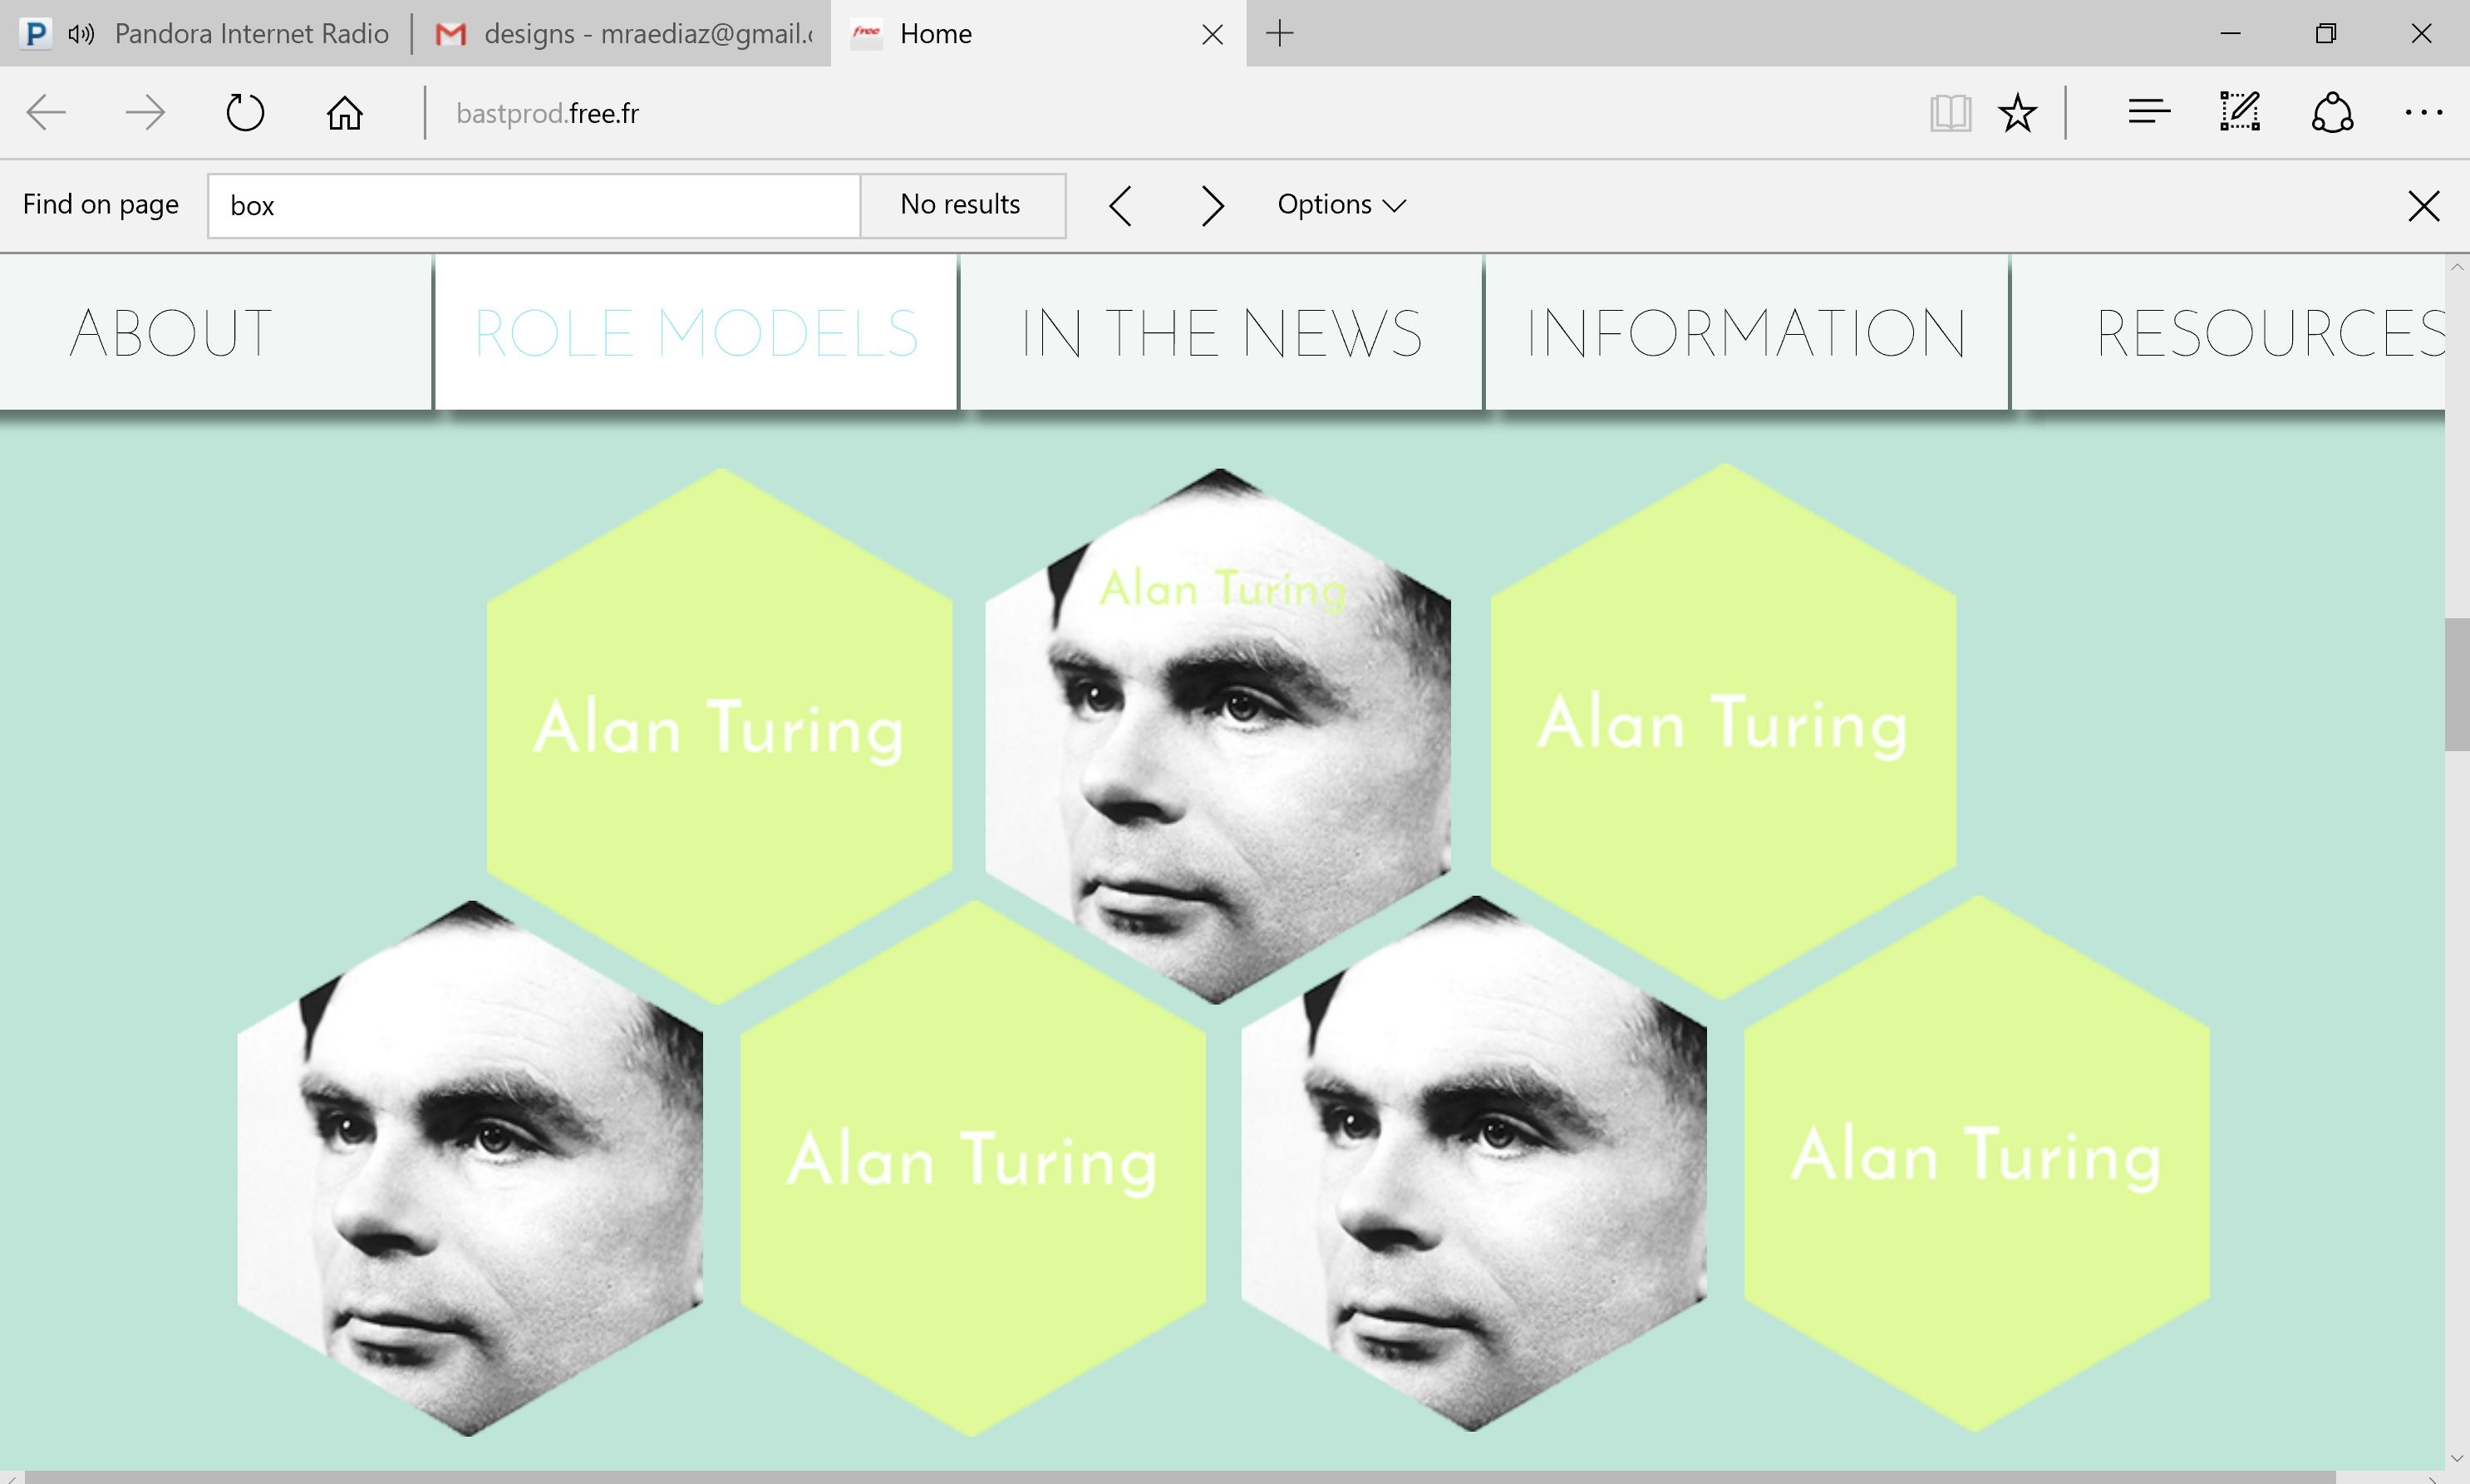
\includegraphics[width=\textwidth,keepaspectratio]{WebsiteDesign}
    					\caption{Website Design Idea}
    				\end{center}
    			\end{figure}
    
    
    As you can see from this picture, I was also hoping to show some other information, such as current events on the topic, information of where to get resources at school (such as TA hours, information on finding a tutor, or office hours for the professors) and a description of the website's mission.\\
    
	Because this idea involved asking for the stories of Kalamazoo College Alumni, I had to go through the Research Ethics Training (or the IRB Application Process) before anything.\footnote{The application can be found in Appendix D.} The process involved preparing the recruitment materials, defining the research methods, and providing a consent form for all of the participants. I had been planning to post a message on the Technology Guild from the Kalamazoo College Linked In connections and sending out emails and personal messages to the alumni I knew. \\
	
		\includepdf[pages={7}]{IRBReport}
		\pagebreak
		
	While I would have preferred to interview each participant individually, I thought an initial start would be best in the form of a survey. In the survey, I was able to receive their official permission to participate, and was able to ask participants questions such as what was their relationship with Computer Science, what had surprised them from the field, and what kept them motivated. \\

	In order to see if this survey would be a successful median to receive entries for the website, I asked my classmates and fellow seniors in our SIP seminar to test-run the survey, and answer it as realistically as possible. Take for example, this entry from Computer Science student, Ariah Lacey:
	
	\begin{quotation}
		\begin{center}
			\singlespacing
			\textit{I was really surprised by the sense of community between programmers/developers/computer scientists surprised me. It's like a big family when you're working on a team, adding to and debugging each other's code. I wish I'd known that earlier or I may have jumped in sooner!}\\
			-Ariah Lacey, class of 2016
		\end{center}
			
	\end{quotation}

	Unfortunately, I was not able to finalize this project, and it had to be closed. \\

I still believe that this is an important idea, and that having a digital connection and support could help anybody feel as if they belong...\\

    \pagebreak
    
    
    
    
    %%%%%%%%%%%%%%%%%%%%%%%%% SUKUMA %%%%%%%%%%%%%%%%%%%%%%%%%%%%%%%%%%%%%%
    
    
    %%%%%%%%%%%%%%%%%%%%%%%%% CLOSING %%%%%%%%%%%%%%%%%%%%%%%%%%%%%%%%%%%%%%
    
    
    
    %%%%%%%%%%%%%%%%%%%%%%%%% APPENDIXES %%%%%%%%%%%%%%%%%%%%%%%%%%%%%%%%%%%%%%
    
	\singlespacing
	\appendices{Appendix A: "The Computer Girls"}{ \section*{Appendix A: "The Computer Girls"}}
	"The Computer Girls," 1967 Cosmopolitan magazine piece about a weird new field, programming, that was dominated by women.An article on women working with technology.\\
	
	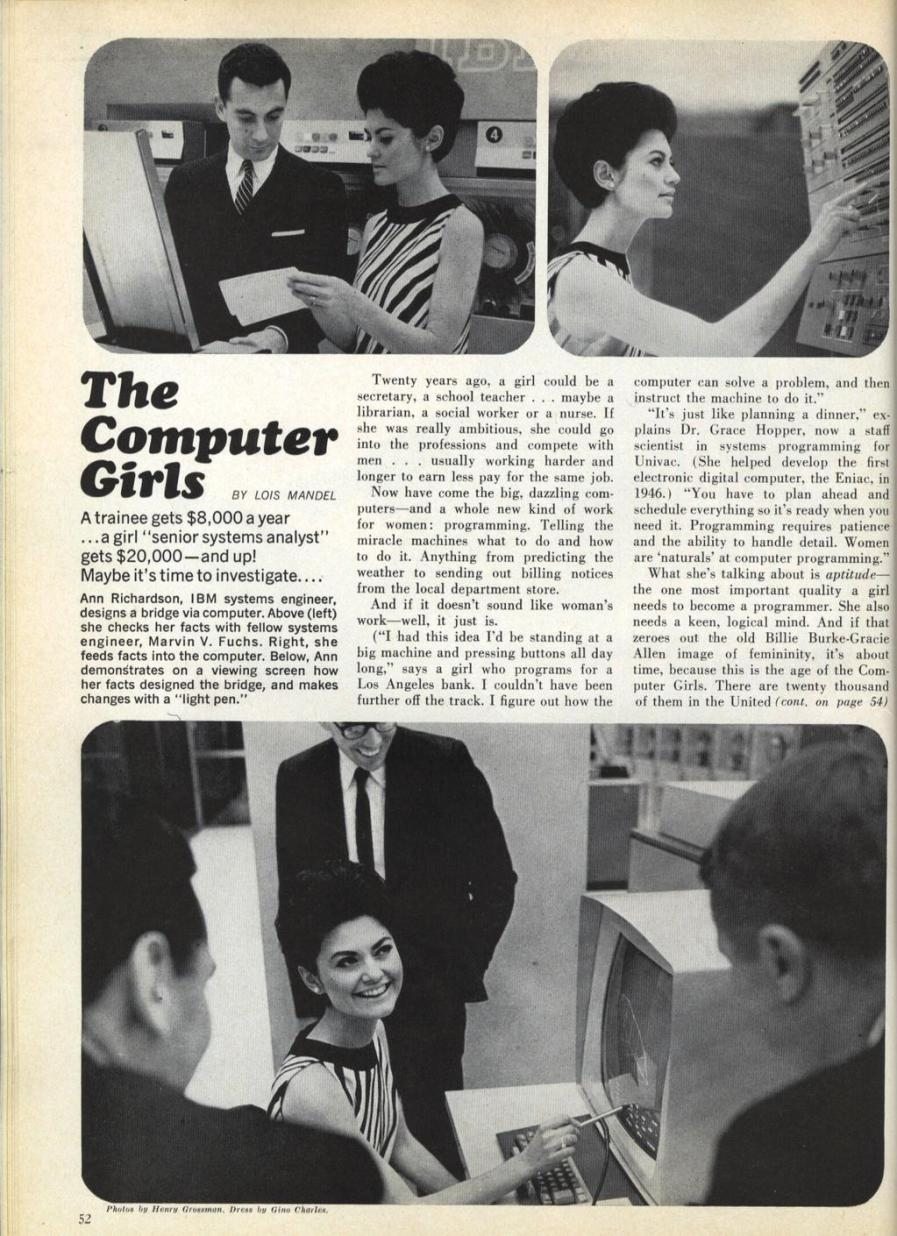
\includegraphics[height=550pt,keepaspectratio]{CosmoPic}
	\pagebreak
	
	
	\appendices{Appendix B: Infographic: Wearable Tech Devices}{\section*{Appendix B: Infographic: Wearable Tech Devices}}
	Infographic: Which Wearable Tech Device Will Win? Demographics and awareness for fitness trackers and smartwatches.\\
	
	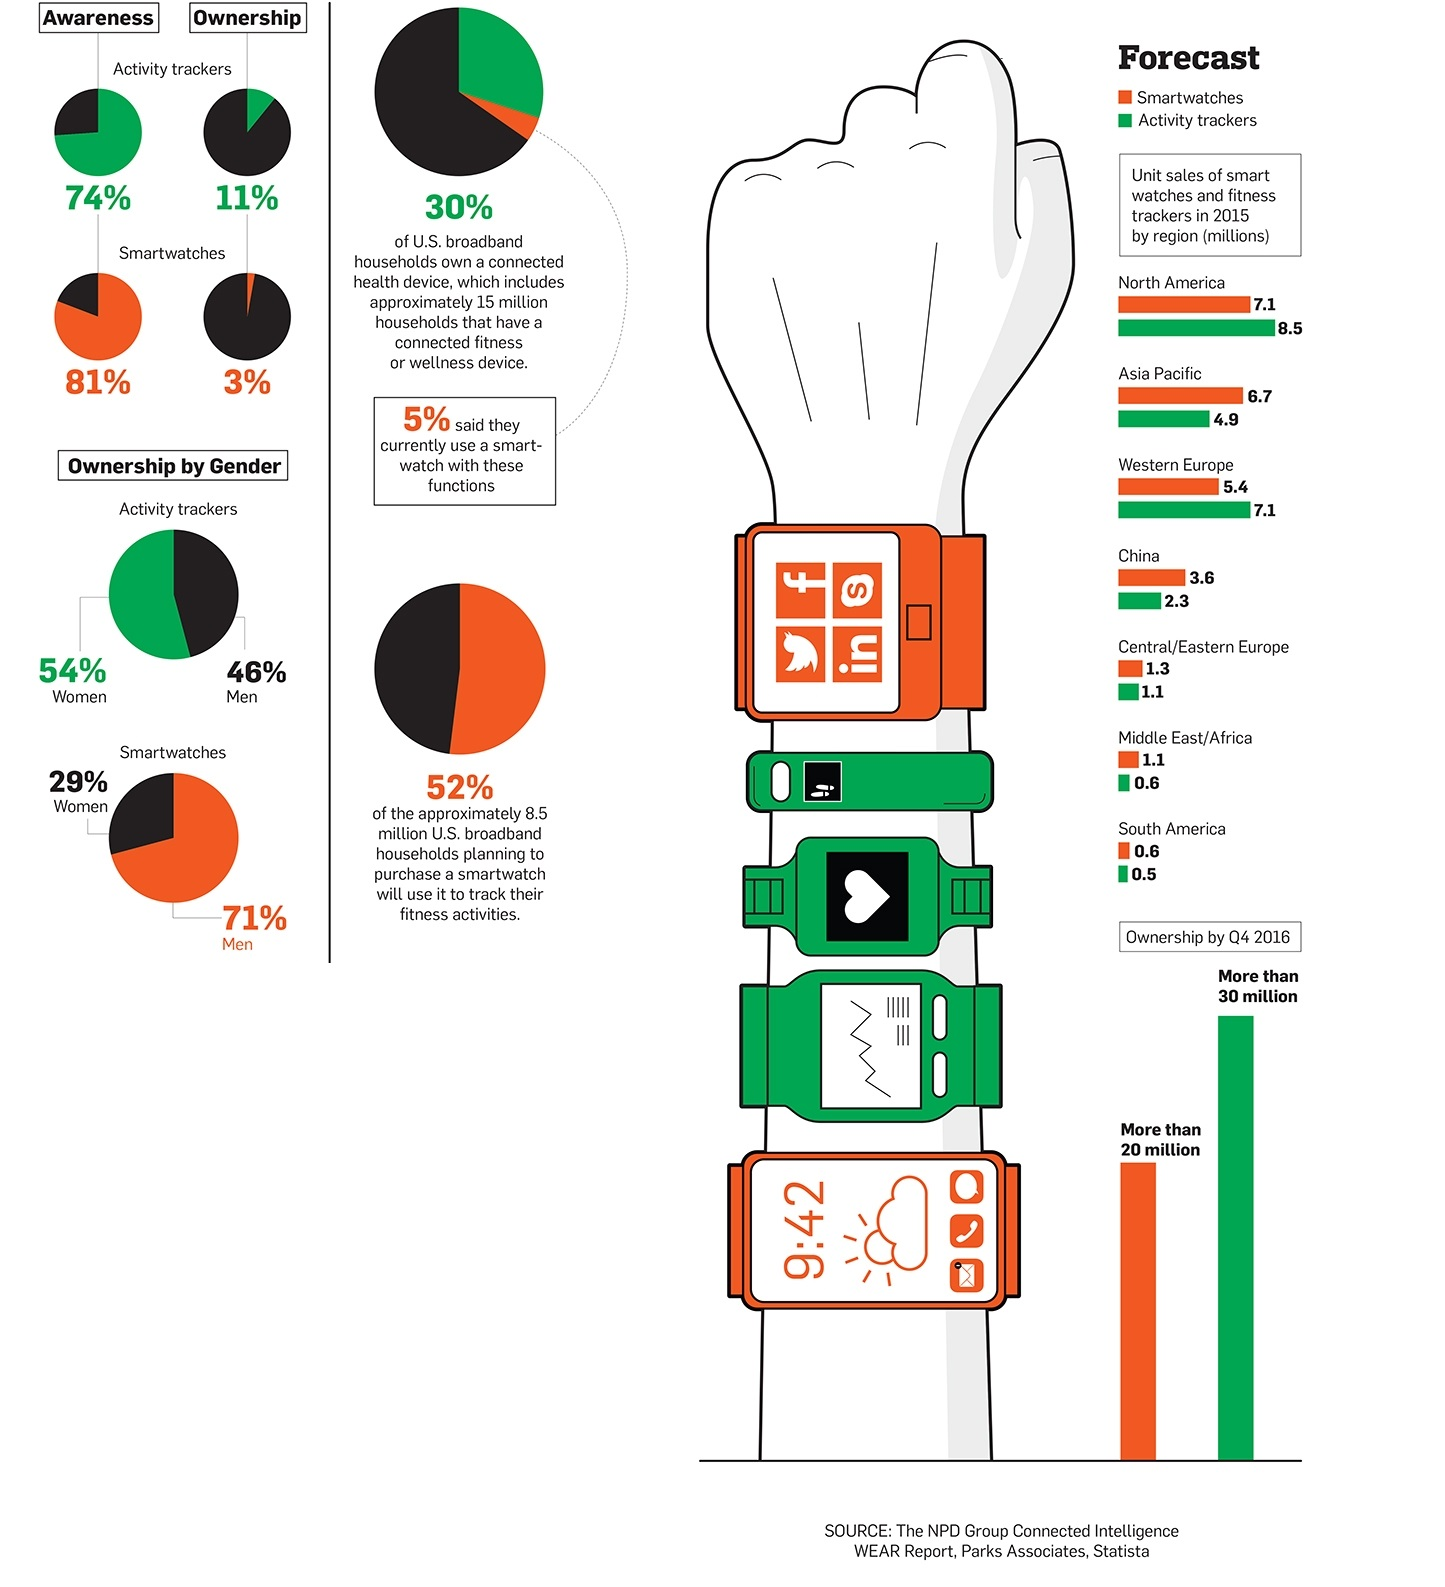
\includegraphics[height=550pt,keepaspectratio]{wearableInfographic}
	\pagebreak
	
	\appendices{Appendix C: Statistics Report of Social Media and Messaging App Users}{\section*{Appendix C: Statistics Report of Social Media and \\Messaging App Users}}
	Exerts from the Pew Research Center Report of mobile messaging and social media use in 2915.
	
	About This Report \\
	This report is a collaborative effort based on the input and analysis of the following individuals. \\
	Find related reports online at pewresearch.org/internet.\\ 
	Maeve Duggan, Research Associate  	 	 \\
	Aaron Smith, Associate Director, Internet, Science, and Technology Research 	 	 	 \\
	Lee Rainie, Director, Internet, Science, and Technology Research  	 	 \\
	Andrew Perrin, Research Assistant  	 	 \\
	Dana Page, Senior Communications Manager 	 	 	\\  
	Margaret Porteus, Information Graphics Designer  	 \\	 	 	 
	Shannon Greenwood, Assistant Digital Producer  	 	 	\\ 	 
	
	
	About Pew Research Center \\
	Pew Research Center is a nonpartisan fact tank that informs the public about the issues, attitudes and trends shaping America and the world. It does not take policy positions. The center conducts public opinion polling, demographic research, content analysis and other data-driven social science research. It studies U.S. politics and policy; journalism and media; Internet, science and technology; religion and public life; Hispanic trends; global attitudes and trends; and U.S. social and demographic trends. All of the center’s reports are available at www.pewresearch.org. Pew Research Center is a subsidiary of The Pew Charitable Trusts, its primary funder. 
	
	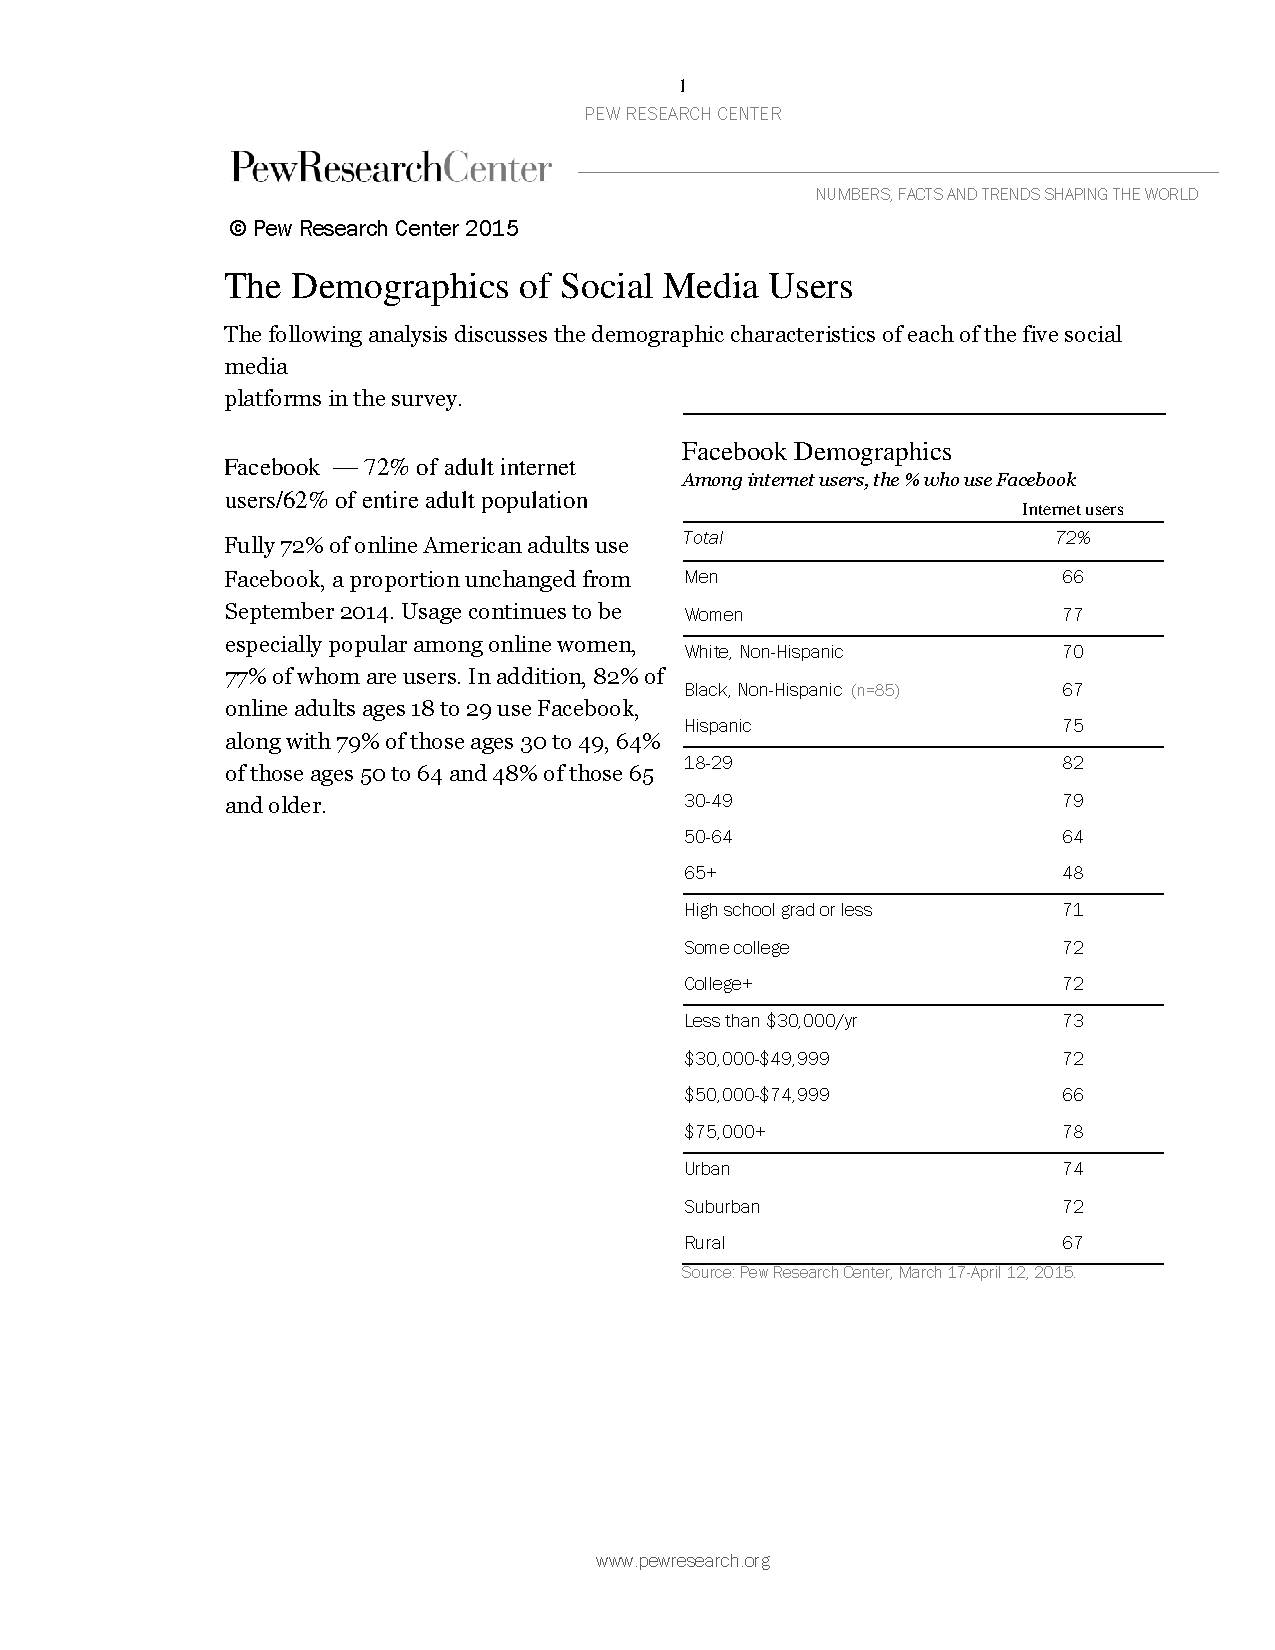
\includepdf[pages={1,2,3,4,5,6,7,8}]{PewReport}
	
	\appendices{Appendix D: Application For IRB Review Of Research With Human Subjects
		}{\section*{Appendix C: Application For IRB Review Of Research With Human Subjects}}
	
	About the Institutional Review Board (IRB) and its application:\\
	
	\begin{quote}
		\justify
		 The first principle of research is to do no harm, however, historically, this principle has not always been followed, thus IRB exists. Doing research, working with human subjects, is a privilege and is one that should not be abused. IRB protects who is being researched, interviewed, observed; IRB also protects the researcher and the institution to which he/she belongs.
	\end{quote}
	
	\bigskip
	This application was started with the hopes of interviewing Kalamazoo College Computer Science alumni in order to create a website connecting students and alumni.
	 
	 
	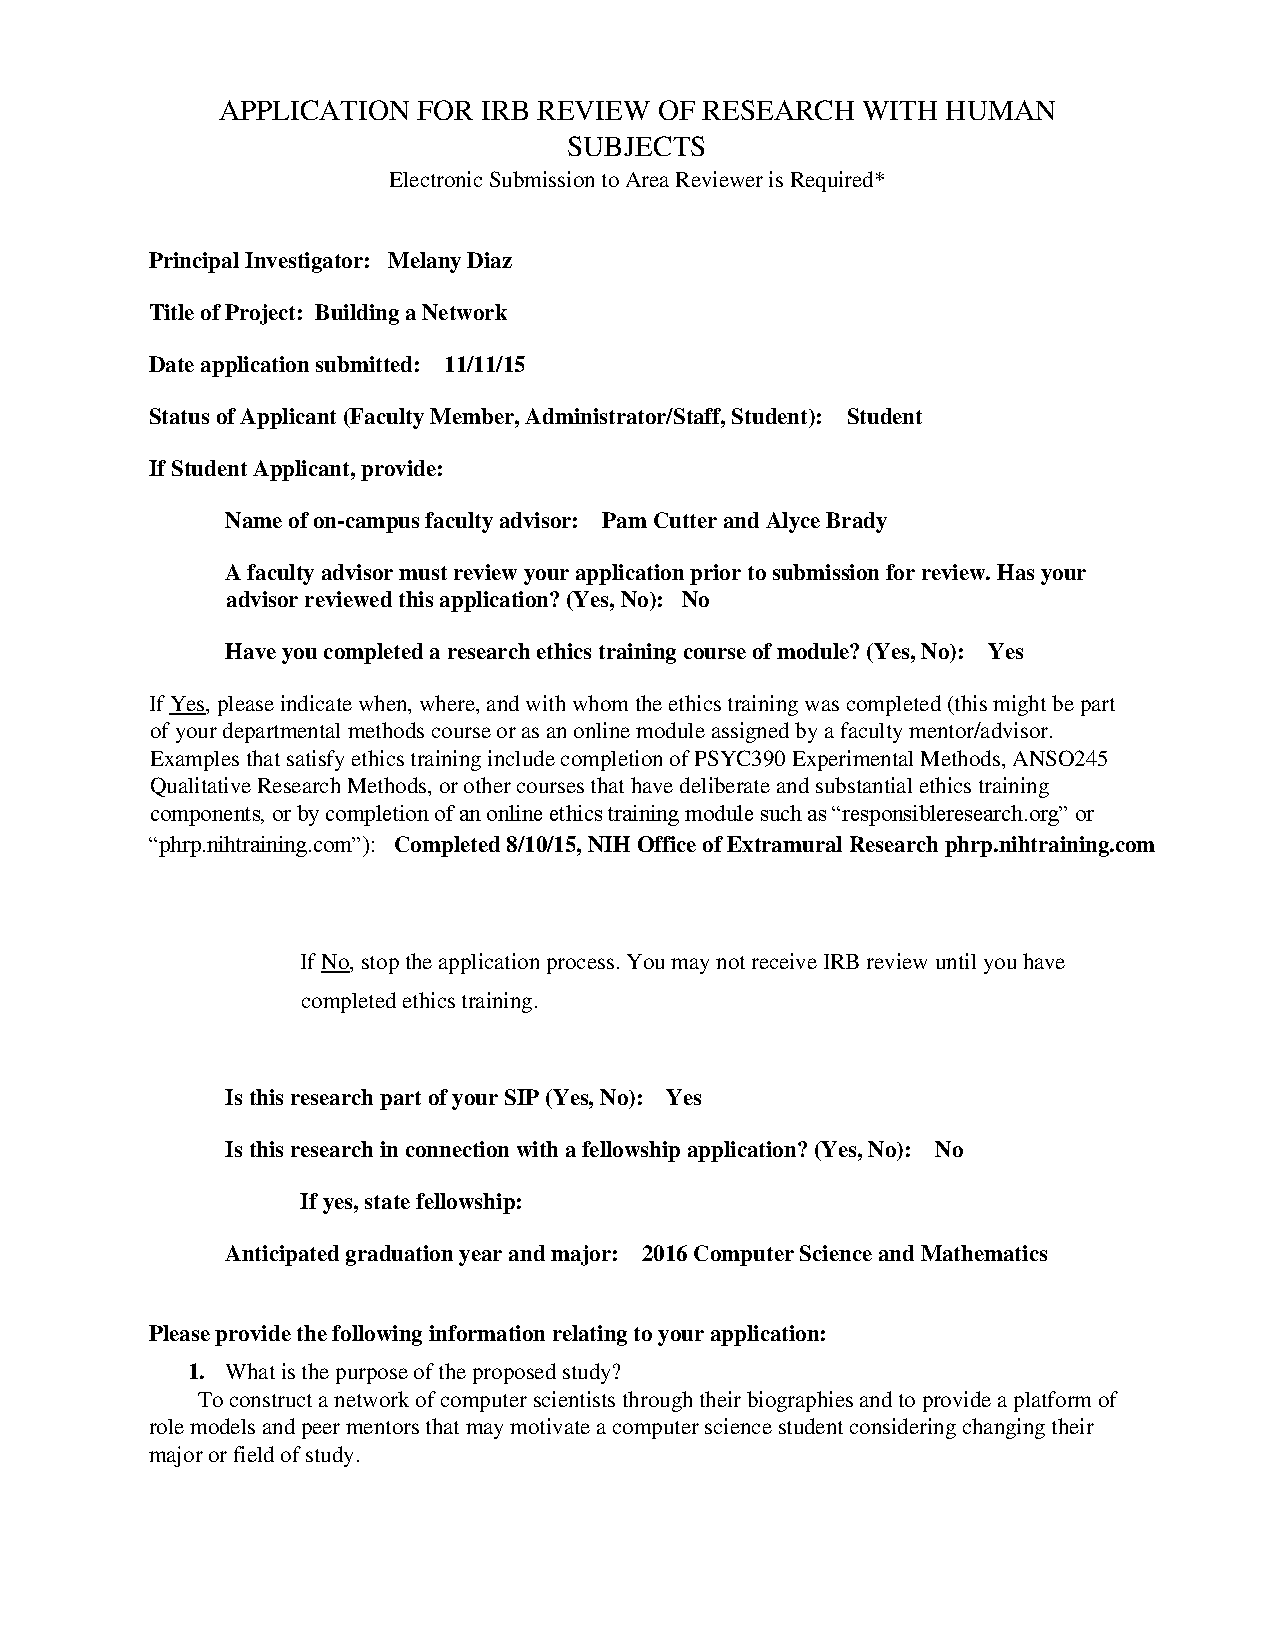
\includepdf[pages={1,2,3,4,5,6,7}]{IRBReport}
	

	
	%%%%%%%%%%%%%%%%%%%%%%%%% BIBLIOGRAPHY %%%%%%%%%%%%%%%%%%%%%%%%%%%%%%%%%%%%%%

	\nocite{*}
	\bibliographystyle{unsrt}
	\bibliography{SipResources}
	
	
	
		


\end{document}

\includegraphics[]{DataToPlot}
\lstinputlisting[language=java, breaklines = true]{insertionSortDecreasing.txt}
